\subsection{Progettazzione di dettaglio}
Si ricorda come l’architettura scelta in IW – Architettura di massima fosse una N-tier con tre strati. Questi sono: DataAccess Layer, BusinessLogic Layer, VMLayer. Nei prossimi capitoli verrà presentato ogni layer in maniera analitica e precisa. In figura \ref{fig:ark-dett-iw} si mostra il diagramma totale che verrà seguito durante la codifica.

\begin{figure}[htbp]
    \centering
    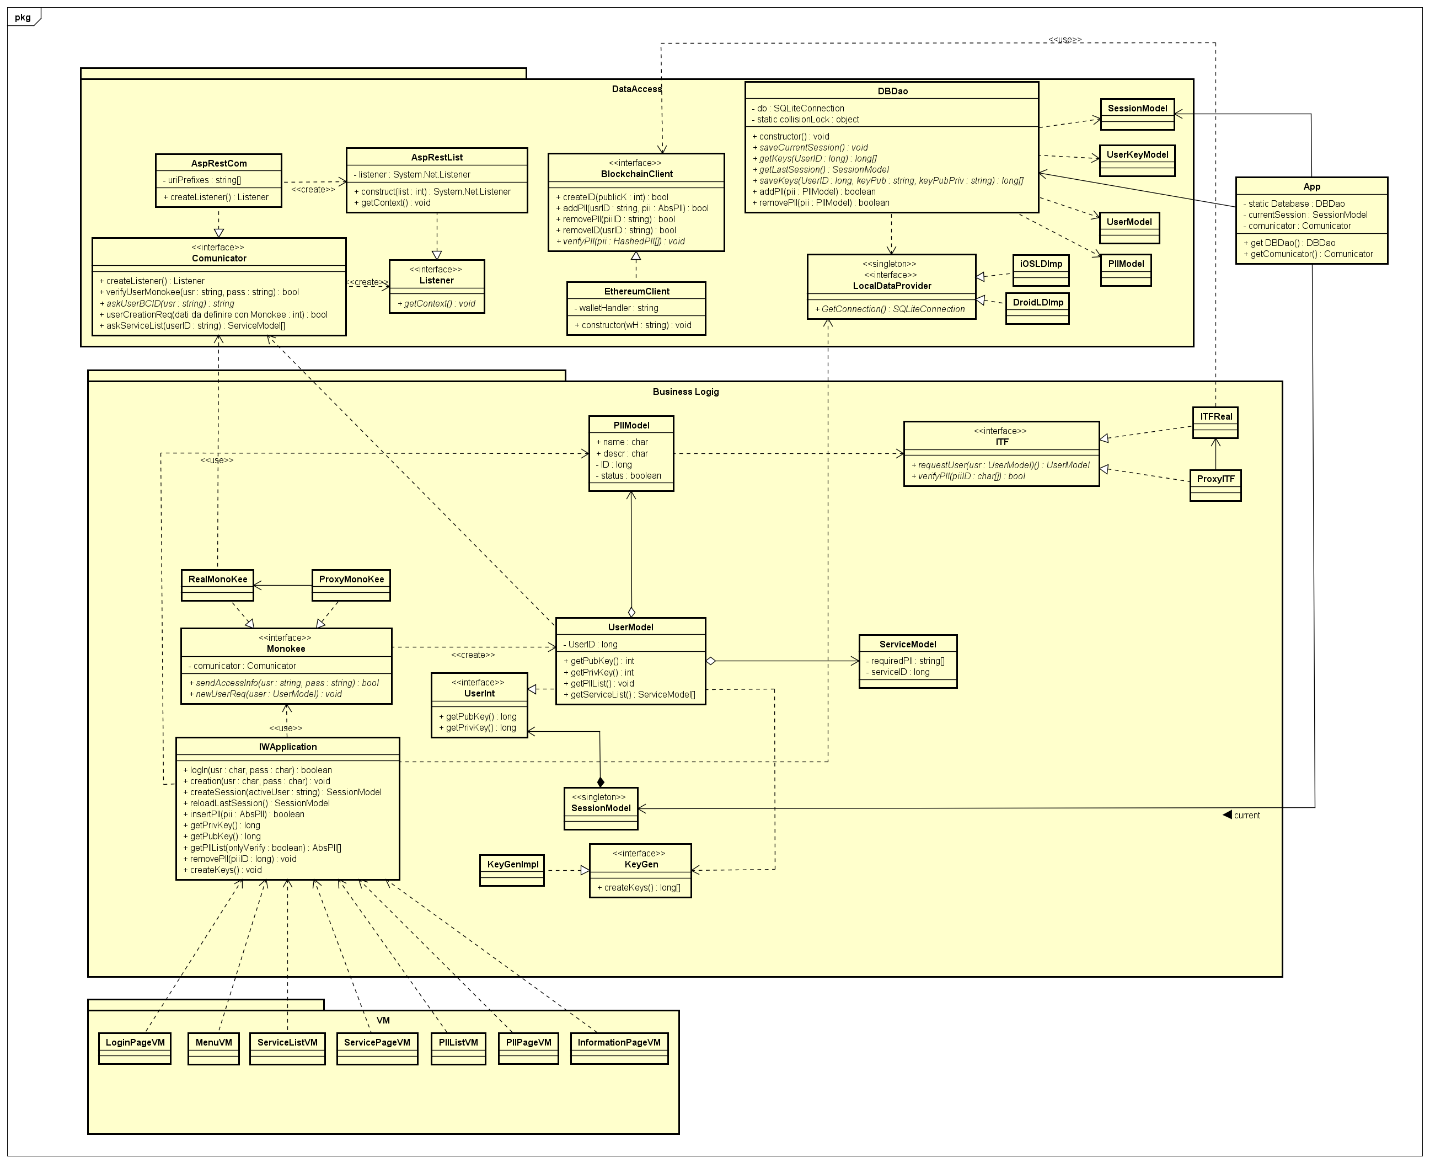
\includegraphics[width=0.9\columnwidth]{iw-complete-uml.png} 
    \caption{Architettura dettagliata IW}
    \label{fig:ark-dett-iw} 
\end{figure}
\subsubsection{DataAccess Layer}
Nel contesto dell’architettura N-tier adottata il BusinessLogic layer è un gruppo di classi che si occupano di interfacciarsi con gli strumenti di persistenza utilizzati dall’applicazione. Questi sono: Monokee (tramite RESTful), ITF e una base di dati locale al dispositivo. 
\begin{figure}[htbp]
    \centering
    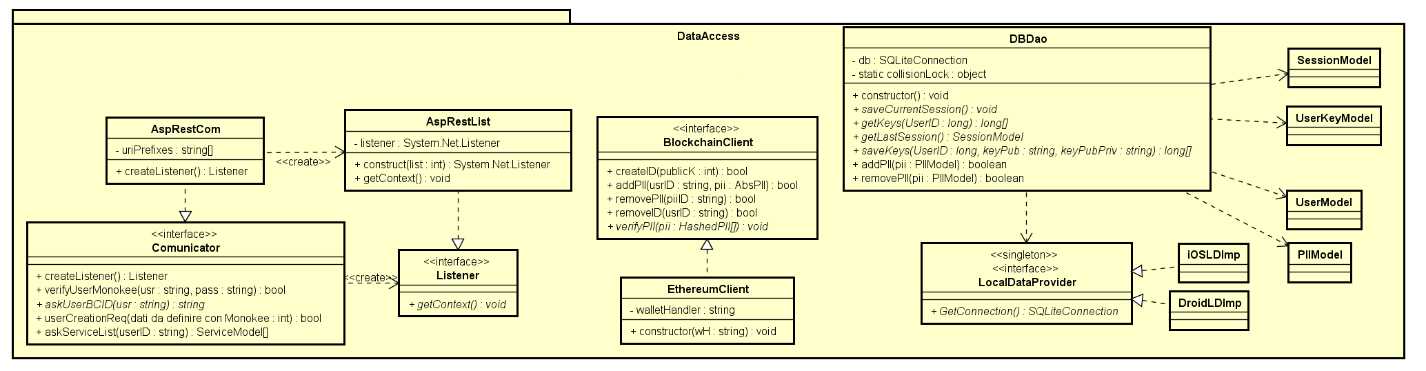
\includegraphics[width=0.9\columnwidth]{dla-iw.png} 
    \caption{Diagramma DataAccess Layer IW}
    \label{fig:dla-iw} 
\end{figure}
\paragraph{Comunicator (interfaccia)}
Questa classe fornisce un’interfaccia per gestire tutte le informazioni attraverso fonti esterne. Deve essere usata per comunicare con Monokee.
\paragraph{Metodi:}

\paragraph{Public Listener createListener()}
\begin{center}
    \begin{longtable}{|p{3cm}|p{9cm}|}%
    \caption{Public Listener createListener()}
    \label{tab:public-void-createListener}
    \endfirsthead
    \endhead
    \hline
    \textbf{Descrizione} & Il metodo ha il compito di restituire un oggetto listener che ascolto le richieste da parte di Monokee.\\
    \hline
    \textbf{Parametri} &  - \\
    \hline
    \textbf{Pseudo Codice} & Non presente \\
    \hline
    \textbf{Note} & - \\
    \hline
    \end{longtable}
    \end{center}


\paragraph{Public bool verifyUserMonokee(usr:string, pass:string)}
\begin{center}
    \begin{longtable}{|p{3cm}|p{9cm}|}%
    \caption{Public Listener createListener()}
    \label{tab:public-bool-verifyUserMonokee}
    \endfirsthead
    \endhead
    \hline
    \textbf{Descrizione} & Il metodo ha il compito di inviare una richiesta a Monokee al fine di verificare i dati forniti dall’utente. Ritorna true le l’autenticazione ha avuto successo altrimenti false.\\
    \hline
    \textbf{Parametri} &      
        \begin{itemize}
            \item usr: string che rappresenta la chiave dell’utente
            \item pass: string che rappresenta la password con cui l’utente usr tenta di effettuare l’accesso. Verificare poi come trasportare la password.
        \end{itemize}
    \\
    \hline
    \textbf{Pseudo Codice} & Non presente \\
    \hline
    \textbf{Note} & - \\
    \hline
    \end{longtable}
    \end{center}






\paragraph{Public string askUserBCID(usr:string)}
\begin{center}
    \begin{longtable}{|p{3cm}|p{9cm}|}%
    \caption{Public string askUserBCID(usr:string)}
    \label{tab:public-string-askUserBCID}
    \endfirsthead
    \endhead
    \hline
    \textbf{Descrizione} & Il metodo ha il compito di inviare una richiesta a Monokee al fine di restituire una stringa contenente l’ID sull’ITFdell’utente.\\
    \hline
    \textbf{Parametri} &      
        \begin{itemize}
            \item usr: string che rappresenta la chiave dell’utente
        \end{itemize}
    \\
    \hline
    \textbf{Pseudo Codice} & Non presente \\
    \hline
    \textbf{Note} & - \\
    \hline
    \end{longtable}
    \end{center}



\paragraph{Public bool userCreationRequest(usr: userModel)}
\begin{center}
    \begin{longtable}{|p{3cm}|p{9cm}|}%
    \caption{Public bool userCreationRequest(usr: userModel)}
    \label{tab:public-bool-userCreationRequest}
    \endfirsthead
    \endhead
    \hline
    \textbf{Descrizione} & Il metodo ha il compito di inviare una richiesta a Monokee al fine creare un utente all’interno del servizio Monokee. Questo metodo invia solo la richiesta e non ha modo di sapere il reale inserimento dell’utente. L’operazione in Monokee non è immediata.\\
    \hline
    \textbf{Parametri} &      
        \begin{itemize}
            \item usr: riferimento ad un oggetto UserModel che contiene i dati che l'utente vuole creare.
        \end{itemize}
    \\
    \hline
    \textbf{Pseudo Codice} & Non presente \\
    \hline
    \textbf{Note} & Non bisogna dare per scontato che la richiesta riceva esito positivo o che venga eseguita in maniera immediata. \\
    \hline
    \end{longtable}
    \end{center}



\paragraph{Public ServiceModel[] getServiceList(usrID:string)}
\begin{center}
    \begin{longtable}{|p{3cm}|p{9cm}|}%
    \caption{Public ServiceModel[] getServiceList(usrID:string)}
    \label{tab:public-ServiceModel[]-getServiceList}
    \endfirsthead
    \endhead
    \hline
    \textbf{Descrizione} & Il metodo ha il compito ritornare la lista dei servizi associati all’utente indicato in Monokee.  \\
    \hline
    \textbf{Parametri} &      
        \begin{itemize}
            \item usrID: stringa che rappresenta la chiave dell’utente in Monokee.
        \end{itemize}
    \\
    \hline
    \textbf{Pseudo Codice} & 
            Var com = App.getComunicator();\newline
            Return serList = await com.askServiceList(this.id);
    \\
    \hline
    \textbf{Note} & Questa informazione deve essere richiesta ogni volta, in quanto l’unico gestore di utenti e servizi e Monokee. \\
    \hline
    \end{longtable}
    \end{center}

\paragraph{AspRestCom (implementa Comunicator)}
\paragraph{Campi dati:}
\begin{itemize}
    \item \textbf{uriPrefixes}: lista stringhe che rappresentano gli uri a cui il listener ascolta. 
\end{itemize}

\paragraph{Metodi:}
\paragraph{Public Listener createListener()}
\begin{center}
    \begin{longtable}{|p{3cm}|p{9cm}|}%
    \caption{Public Listener createListener()}
    \label{tab:public-listner-createListener}
    \endfirsthead
    \endhead
    \hline
    \textbf{Descrizione} & Il metodo ha il compito di restituire un oggetto listener che ascolto le richieste da parte di Monokee.  \\
    \hline
    \textbf{Parametri} &      
        -
    \\
    \hline
    \textbf{Pseudo Codice} & 
        check (uriPrefixes not null); \newline
        check(uriPrefixes not empty) \newline
        listener = HttpListener; \newline
        foreach (uri in uriPrefixes) {
            listener.add(uri); \newline
        }
        listener.start(); \newline
        return new AspRest( listener); \newline
    \\
    \hline
    \textbf{Note} & - \\
    \hline
    \end{longtable}
    \end{center}

\paragraph{Public bool verifyUserMonokee(usr:string, pass:string)}
\begin{center}
    \begin{longtable}{|p{3cm}|p{9cm}|}%
    \caption{Public bool verifyUserMonokee(usr:string, pass:string)}
    \label{tab:public-bool-verifyUserMonokeeImpl}
    \endfirsthead
    \endhead
    \hline
    \textbf{Descrizione} & Il metodo ha il compito di inviare una richiesta a Monokee al fine di verificare i dati forniti dall’utente. Ritorna true le l’autenticazione ha avuto successo altrimenti false.  \\
    \hline
    \textbf{Parametri} &      
        \begin{itemize}
            \item usr: long che rappresenta la chiave dell’utente
            \item pass: string che rappresenta la password con cui l’utente usr tenta di effettuare l’accesso. Verificare poi come trasportare la password.
        \end{itemize}
    \\
    \hline
    \textbf{Pseudo Codice} & 
    string content =” accessReq”+usr+pass; \newline
    ASCIIEncoding encoding=new ASCIIEncoding(); \newline
    byte[]  buffer =encoding.GetBytes(content); \newline
    request.ContentType="application/x-www-IWAccessRequest "; \newline
    request.ContentLength=content.Length; \newline
    Stream newStream=request.GetRequestStream(); \newline
    newStream.Write(buffer,0,buffer.Length); \newline
    newStream.Close();
    \\
    \hline
    \textbf{Note} & \url{http://www.dotnethell.it/tips/SendPOSTHttp.aspx} \\
    \hline
    \end{longtable}
    \end{center}


    \paragraph{Public string askUserBCID(usr:string)}
    \begin{center}
        \begin{longtable}{|p{3cm}|p{9cm}|}%
        \caption{Public string askUserBCID(usr:string)}
        \label{tab:public-string-askUserBCIDImpl}
        \endfirsthead
        \endhead
        \hline
        \textbf{Descrizione} & Il metodo ha il compito di inviare una richiesta a Monokee al fine di restituire una stringa contenente l’ID sull’ITF dell’utente. \\
        \hline
        \textbf{Parametri} &      
            \begin{itemize}
                \item usr: string che rappresenta la chiave dell’utente
            \end{itemize}
        \\
        \hline
        \textbf{Pseudo Codice} & 
        string content =”ITF ID request”+usr;\newline
        ASCIIEncoding encoding=new ASCIIEncoding();\newline
        byte[]  buffer =encoding.GetBytes(content);\newline
        request.ContentType="application/x-www-ITFIDrequest ";\newline.
        request.ContentLength=content.Length;\newline
        Stream newStream=request.GetRequestStream();\newline
        newStream.Write(buffer,0,buffer.Length);\newline
        newStream.Close();\newline
        if (response != no pass) return response;\newline
        else return null;\newline
        \\
        \hline
        \textbf{Note} & \url{http://www.dotnethell.it/tips/SendPOSTHttp.aspx} \\
        \hline
        \end{longtable}
        \end{center}


    \paragraph{Public bool userCreationRequest(usr: userModel)}
    \begin{center}
        \begin{longtable}{|p{3cm}|p{9cm}|}%
        \caption{Public bool userCreationRequest(usr: userModel)}
        \label{tab:public-boll-userCreationRequestImpl}
        \endfirsthead
        \endhead
        \hline
        \textbf{Descrizione} & Il metodo ha il compito di inviare una richiesta a Monokee al fine creare un utente all’interno del servizio Monokee. Questo metodo invia solo la richiesta e non ha modo di sapere il reale inserimento dell’utente. L’operazione in Monokee non è immediata. \\
        \hline
        \textbf{Parametri} &      
            \begin{itemize}
                \item usr: riferimento ad un oggetto UserModel che contiene i dati che l'utente vuole creare.
            \end{itemize}
        \\
        \hline
        \textbf{Pseudo Codice} & 
        string content =”Monokee user creation request”+usr;\newline
        ASCIIEncoding encoding=new ASCIIEncoding();\newline
        byte[]  buffer =encoding.GetBytes(content);\newline
        request.ContentType="application/x-www-MONK-creationReq ";\newline.
        request.ContentLength=content.Length;\newline
        Stream newStream=request.GetRequestStream();\newline
        newStream.Write(buffer,0,buffer.Length);\newline
        newStream.Close();\newline
        if (response != no pass) return response;\newline
        else return null;\newline
        \\
        \hline
        \textbf{Note} & Non bisogna dare per scontato che la richiesta riceva esito positivo o che venga eseguita in maniera immediata. \\
        \hline
        \end{longtable}
        \end{center}

\paragraph{Listener (interfaccia)}
È un oggetto con il compito di rimanere in ascolto su determinati uri. È un oggetto non mutabile.
\paragraph{Metodi:}
\paragraph{Public void getContext()}
    \begin{center}
        \begin{longtable}{|p{3cm}|p{9cm}|}%
        \caption{Public void getContext()}
        \label{tab:public-void-getContext}
        \endfirsthead
        \endhead
        \hline
        \textbf{Descrizione} & Il metodo ha il compito di ritornare appena arriva un messaggio inviato da uno degli uri specificati nella AspRestComp. \\
        \hline
        \textbf{Parametri} &      
            -
        \\
        \hline
        \textbf{Pseudo Codice} & 
         Non presente \\
        \hline
        \textbf{Note} & - \\
        \hline
        \end{longtable}
        \end{center}


\paragraph{AspRestList (implementa Listerner)}
È un oggetto con il compito di rimanere in ascolto su determinati uri. È un oggetto non mutabile. Questa classe rappresenta un wrapper del listener di \emph{System.Net}.
\paragraph{Campi dati:}
\begin{itemize}
    \item listener: è il listener fornito dal System.Net. Creato da AspRestComp
\end{itemize}

\paragraph{Metodi:}
\paragraph{Public constructor()}
    \begin{center}
        \begin{longtable}{|p{3cm}|p{9cm}|}%
        \caption{Public constructor()}
        \label{tab:public-list-constructor}
        \endfirsthead
        \endhead
        \hline
        \textbf{Descrizione} & Il metodo ha il compito di costruire l’oggetto Listener da un’istanza del listener fornito da System.Net \\
        \hline
        \textbf{Parametri} &      
            \begin{itemize}
                \item List: è un’implementazione di System.Net listener.
            \end{itemize}
        \\
        \hline
        \textbf{Pseudo Codice} & 
            This.listener = List; \\
        \hline
        \textbf{Note} & - \\
        \hline
        \end{longtable}
        \end{center}


\paragraph{Public void getContext()}
\begin{center}
    \begin{longtable}{|p{3cm}|p{9cm}|}%
    \caption{Public void getContext()}
    \label{tab:public-void-getContextImpl}
    \endfirsthead
    \endhead
    \hline
    \textbf{Descrizione} & Il metodo ha il compito di ritornare appena arriva un messaggio inviato da uno degli uri specificati nella AspRestComp. \\
    \hline
    \textbf{Parametri} &      
     - \\
    \hline
    \textbf{Pseudo Codice} & 
    Listener.getContext();\\
    \hline
    \textbf{Note} & - \\
    \hline
    \end{longtable}
    \end{center}


\paragraph{BlockchainClient (interfaccia)}
Questa interfaccia ha il compito di rappresentare un canale di comunicazione verso gli SmartContract. Deve essere atea rispetto alla tipologia di \gls{blockchaing} usata.

\paragraph{Metodi:}
\paragraph{public bool verifyPII(pii: HashedPII[])}
\begin{center}
    \begin{longtable}{|p{3cm}|p{9cm}|}%
    \caption{public bool verifyPII(pii: HashedPII[])}
    \label{tab:public-bool-verifyPII}
    \endfirsthead
    \endhead
    \hline
    \textbf{Descrizione} & Il metodo ha il compito di chiamare il metodo presente negli smartContract che verifica i dati. \\
    \hline
    \textbf{Parametri} &      
    \begin{itemize}
        \item pii: è una lista di oggetti hashedPII da verificare nell’ITF.
    \end{itemize} 
    \\
    \hline
    \textbf{Pseudo Codice} & 
    Non presente\\
    \hline
    \textbf{Note} & L’implementazione sarà sensibilmente diversa in base alla specifica blockchain usata. \\
    \hline
    \end{longtable}
    \end{center}

\paragraph{public bool createID(publicK : long)}
\begin{center}
    \begin{longtable}{|p{3cm}|p{9cm}|}%
    \caption{public bool createID(publicK : long)}
    \label{tab:public-bool-createID}
    \endfirsthead
    \endhead
    \hline
    \textbf{Descrizione} & Il metodo ha il compito di chiamare il metodo presente negli smartContract che inserisce un utente nell’ITF. \\
    \hline
    \textbf{Parametri} &      
    \begin{itemize}
        \item publicK: è un long che rappresenta la chiave pubblica dell’utente creato. La chiave privata deve rimanere solo in locale nell’IW.
    \end{itemize} 
    \\
    \hline
    \textbf{Pseudo Codice} & 
    Non presente\\
    \hline
    \textbf{Note} & L’implementazione sarà sensibilmente diversa in base alla specifica blockchain usata. \\
    \hline
    \end{longtable}
    \end{center}

\paragraph{public bool addPII(usrID:string, pii:AbsPII)}
\begin{center}
    \begin{longtable}{|p{3cm}|p{9cm}|}%
    \caption{public bool addPII(usrID:string, pii:AbsPII)}
    \label{tab:public-bool-addPII}
    \endfirsthead
    \endhead
    \hline
    \textbf{Descrizione} & Il metodo ha il compito di chiamare il metodo presente negli smartContract che inserisce una nuova PII ad un utente.\\
    \hline
    \textbf{Parametri} &      
    \begin{itemize}
        \item usrID: è una stringa che rappresenta la chiave pubblica dell’utente a cui si vuole creare.
        \item Pii: è una lista di oggetti AbsPII che si vuole aggiungere all’utente identificato dalla chiave.
    \end{itemize} 
    \\
    \hline
    \textbf{Pseudo Codice} & 
    Non presente\\
    \hline
    \textbf{Note} & L’implementazione sarà sensibilmente diversa in base alla specifica blockchain usata. \\
    \hline
    \end{longtable}
    \end{center}


\paragraph{public bool removePII(piiID:string)}
\begin{center}
    \begin{longtable}{|p{3cm}|p{9cm}|}%
    \caption{public bool removePII(piiID:string)}
    \label{tab:public-bool-removePII}
    \endfirsthead
    \endhead
    \hline
    \textbf{Descrizione} & Il metodo ha il compito di chiamare il metodo presente negli smartContract che elimina una determinata PII ad un utente.\\
    \hline
    \textbf{Parametri} &      
    \begin{itemize}
        \item piiID: è una stringa che rappresenta la chiave della PII che si vuole elimare.
    \end{itemize} 
    \\
    \hline
    \textbf{Pseudo Codice} & 
    Non presente\\
    \hline
    \textbf{Note} & L’implementazione sarà sensibilmente diversa in base alla specifica blockchain usata. \\
    \hline
    \end{longtable}
    \end{center}

\paragraph{public bool removeID(usrID:string)}
\begin{center}
    \begin{longtable}{|p{3cm}|p{9cm}|}%
    \caption{public bool removeID(usrID:string)}
    \label{tab:public-bool-removeID}
    \endfirsthead
    \endhead
    \hline
    \textbf{Descrizione} & Il metodo ha il compito di chiamare il metodo presente negli smartContract che elimina un determinato utente.\\
    \hline
    \textbf{Parametri} &      
    \begin{itemize}
        \item usrID: è una stringa che rappresenta la chiave dell’utente che si vuole eliminare.
    \end{itemize} 
    \\
    \hline
    \textbf{Pseudo Codice} & 
    Non presente\\
    \hline
    \textbf{Note} & L’implementazione sarà sensibilmente diversa in base alla specifica blockchain usata. \\
    \hline
    \end{longtable}
    \end{center}
    
\paragraph{NethereumClient (implementa BlockchainClient)}
Questa classe rappresentare un canale di comunicazione verso gli \gls{SmartContractg} di una rete Ethereum. Fa uso della libreria .NET Nethereum per instaurare la comunicazione. 
\paragraph{Campi dati}
\begin{itemize}
    \item walletHandler: è una stringa che rappresenta l’indirizzo del contratto WalletHandler all’interno della blockchain. 
\end{itemize}
\paragraph{Metodi:}


\paragraph{public constructor(walletHandler: string)}
\begin{center}
    \begin{longtable}{|p{3cm}|p{9cm}|}%
    \caption{public constructor(walletHandler: string)}
    \label{tab:public-nethclient-constructor}
    \endfirsthead
    \endhead
    \hline
    \textbf{Descrizione} & Il metodo ha il compito di costruire l’oggetto Ethereum client.\\
    \hline
    \textbf{Parametri} &      
    \begin{itemize}
        \item walletHandler: è una stringa che rappresenta l’indirizzo del contratto WalletHandler.
    \end{itemize} 
    \\
    \hline
    \textbf{Pseudo Codice} & 
    This.walletHandler = walletHandler;\\
    \hline
    \textbf{Note} & - \\
    \hline
    \end{longtable}
    \end{center}


\paragraph{Public bool verifyPII(pii: HashedPII[])}
\begin{center}
    \begin{longtable}{|p{3cm}|p{9cm}|}%
    \caption{Public bool verifyPII(pii: HashedPII[])}
    \label{tab:public-bool-verifyPIIImpl}
    \endfirsthead
    \endhead
    \hline
    \textbf{Descrizione} & Il metodo ha il compito di chiamare il metodo presente negli smartContract che verifica i dati.\\
    \hline
    \textbf{Parametri} &      
    \begin{itemize}
        \item pii: è una lista di oggetti hashedPII da verificare nell’ITF.
    \end{itemize} 
    \\
    \hline
    \textbf{Pseudo Codice} & 
    Nethereum.Web3.Web3();\newline
    web3. Eth. Transactions.verifyMethod.Call;\newline
    web3. Eth. Transactions.GetTransactionReceipt;\newline
    return result;\newline
    \\
    \hline
    \textbf{Note} & \url{http://nethereum.com/} \\
    \hline
    \end{longtable}
    \end{center}

\paragraph{public bool createID(publicK : long)}
\begin{center}
    \begin{longtable}{|p{3cm}|p{9cm}|}%
    \caption{public bool createID(publicK : long)}
    \label{tab:public-bool-createIDImpl}
    \endfirsthead
    \endhead
    \hline
    \textbf{Descrizione} & Il metodo ha il compito di chiamare il metodo presente negli smartContract che inserisce un utente nell’ITF.\\
    \hline
    \textbf{Parametri} &      
    \begin{itemize}
        \item publicK: è un long che rappresenta la chiave pubblica dell’utente creato. La chiave privata deve rimanere solo in locale nell’IW.
    \end{itemize} 
    \\
    \hline
    \textbf{Pseudo Codice} & 
    Nethereum.Web3.Web3();\newline
    trova abi;\newline
    var contract = web3.Eth.GetContract(abi, walletHandler);\newline
    var createFunction = contract.GetFunction("createUser");\newline
    var result = await createFunction.CallAsync<string>(id);\newline
    \\
    \hline
    \textbf{Note} & \url{http://nethereum.com/} \\
    \hline
    \end{longtable}
    \end{center}


\paragraph{public bool createID(publicK : long)}
\begin{center}
    \begin{longtable}{|p{3cm}|p{9cm}|}%
    \caption{public bool createID(publicK : long)}
    \label{tab:public-bool-createIDImpl}
    \endfirsthead
    \endhead
    \hline
    \textbf{Descrizione} & Il metodo ha il compito di chiamare il metodo presente negli smartContract che inserisce un utente nell’ITF.\\
    \hline
    \textbf{Parametri} &      
    \begin{itemize}
        \item publicK: è un long che rappresenta la chiave pubblica dell’utente creato. La chiave privata deve rimanere solo in locale nell’IW.
    \end{itemize} 
    \\
    \hline
    \textbf{Pseudo Codice} & 
    Nethereum.Web3.Web3();\newline
    trova abi;\newline
    var contract = web3.Eth.GetContract(abi, walletHandler);\newline
    var createFunction = contract.GetFunction("createUser");\newline
    var result = await createFunction.CallAsync<string>(id);\newline
    \\
    \hline
    \textbf{Note} & \url{http://nethereum.com/} \\
    \hline
    \end{longtable}
    \end{center}


\paragraph{public bool addPII(usrID:string, pii:AbsPII)}
\begin{center}
    \begin{longtable}{|p{3cm}|p{9cm}|}%
    \caption{public bool addPII(usrID:string, pii:AbsPII)}
    \label{tab:public-bool-addPIIImpl}
    \endfirsthead
    \endhead
    \hline
    \textbf{Descrizione} & Il metodo ha il compito di chiamare il metodo presente negli smartContract che inserisce una nuova PII ad un utente.\\
    \hline
    \textbf{Parametri} &      
    \begin{itemize}
        \item usrID: è una stringa che rappresenta la chiave pubblica dell’utente a cui si vuole creare.
        \item Pii: è una lista di oggetti AbsPII che si vuole aggiungere all’utente identificato dalla chiave.
    \end{itemize} 
    \\
    \hline
    \textbf{Pseudo Codice} & 
    Nethereum.Web3.Web3();\newline
    Trova abi;\newline 
    Var contract= web3.Eth.GetContract(abi, walletHandler);\newline
    Var addPIIFunction =  contract.GetFunction(“addPII”);\newline
    Var result = await addPIIFunction.CallAsync<PII>(pii);\newline
    \\
    \hline
    \textbf{Note} & \url{http://nethereum.com/}, la chiave deve essere fornita in quanto questa verrà usata anche nel contesto dell’ITF. \\
    \hline
    \end{longtable}
    \end{center}



\paragraph{public bool removePII(piiID:string)}
\begin{center}
    \begin{longtable}{|p{3cm}|p{9cm}|}%
    \caption{public bool removePII(piiID:string)}
    \label{tab:public-bool-removePIIImpl}
    \endfirsthead
    \endhead
    \hline
    \textbf{Descrizione} & Il metodo ha il compito di chiamare il metodo presente negli smartContract che elimina una determinata PII ad un utente.\\
    \hline
    \textbf{Parametri} &      
    \begin{itemize}
        \item piiID: è una stringa che rappresenta la chiave della PII che si vuole elimare.
    \end{itemize} 
    \\
    \hline
    \textbf{Pseudo Codice} & 
    Nethereum.Web3.Web3();\newline
    trova abi(walletHandler);\newline
    var contract = web3.Eth.GetContract(abi, walletHandler);\newline
    var removeFuncition = contract.GetFunction(“removePII”);\newline
    var result = await removeFunction.CallAsync<string>(piiID);\newline
    \\
    \hline
    \textbf{Note} & \url{http://nethereum.com/}\\
    \hline
    \end{longtable}
    \end{center}

\paragraph{public bool removeID(usrID:string)}
\begin{center}
    \begin{longtable}{|p{3cm}|p{9cm}|}%
    \caption{public bool removeID(usrID:string)}
    \label{tab:public-bool-removeIDImpl}
    \endfirsthead
    \endhead
    \hline
    \textbf{Descrizione} & Il metodo ha il compito di chiamare il metodo presente negli smartContract che elimina un determinato utente.\\
    \hline
    \textbf{Parametri} &      
    \begin{itemize}
        \item usrID: è una stringa che rappresenta la chiave dell’utente che si vuole eliminare.
    \end{itemize} 
    \\
    \hline
    \textbf{Pseudo Codice} & 
    Nethereum.Web3.Web3();\newline
    trova abi(walletHandler);\newline
    var contract = web3.Eth.GetContract(abi, walletHandler);\newline
    var removeFuncition = contract.GetFunction(“removeID”);\newline
    var result = await removeFunction.CallAsync<string>(usrID);\newline
    \\
    \hline
    \textbf{Note} & \url{http://nethereum.com/}\\
    \hline
    \end{longtable}
    \end{center}

\paragraph{DBDao}
Questa classe ha il compito di fare da tramite per gli accessi al database. Rappresenta quindi il data access object relativo al database. Per effettuare la connessione viene usata la classe LocalDataProvider.
\paragraph{Campi dati:}
\begin{itemize}
    \item database: è un oggetto di tipo SQLiteConnection che rappresenta la connessione con il database
    \item static collisionLock: è un oggetto di qualsiasi tipo con lo scopo di fornire un lock all’oggetto per non permettere usi concorrenti della risorsa.
\end{itemize}

\paragraph{Metodi:}


\paragraph{public constructor()}
\begin{center}
    \begin{longtable}{|p{3cm}|p{9cm}|}%
    \caption{public constructor()}
    \label{tab:public-dao-constructor}
    \endfirsthead
    \endhead
    \hline
    \textbf{Descrizione} & Il metodo ha il compito costruire l’oggetto DBDao\\
    \hline
    \textbf{Parametri} &      
    -
    \\
    \hline
    \textbf{Pseudo Codice} & 
    database = DependencyService.Get<IRecipesDatabaseConnection>().GetConnection();\newline
    database.CreateTable<PIIModel>();\newline
    database.CreateTable<SessionModel>();\newline
    database.CreateTable<UserModel>();\newline
    \\
    \hline
    \textbf{Note} & 
    Questo metodo deve essere chiamato nella classe App del progetto nel seguente modo. 
    public static DBDao Database \newline
    { \newline
        get \newline
        { \newline
            if (database == null) \newline
            { \newline
                database = new DBDao(); \newline
            }
            return database;\newline
        }\newline
    }\newline
    Questo serve per creare l’unica istanza della base di dati all’avvio dell’applicazione.
    \\
    \hline
    \end{longtable}
    \end{center}


\paragraph{public saveCurrentSession()}
\begin{center}
    \begin{longtable}{|p{3cm}|p{9cm}|}%
    \caption{public saveCurrentSession()}
    \label{tab:public-savecurrentsession}
    \endfirsthead
    \endhead
    \hline
    \textbf{Descrizione} & Il metodo ha il compito salvare all’interno del database la sessione corrente\\
    \hline
    \textbf{Parametri} &      
    -
    \\
    \hline
    \textbf{Pseudo Codice} & 
    var sessionModel = ((IW)Application).currentSession;\newline
    lock (collisionLock)\newline
    {\newline
        if (sessionModel.Id != 0)\newline
        {\newline
            database.Update(sessionModel);\newline
            return sessionModel.Id;\newline
        }\newline
        else\newline
        {\newline
            return database.Insert(sessionModel);\newline
        }\newline
    }\newline
    \\
    \hline
    \textbf{Note} & 
    Il controllo è utile nel contesto in cui id è auto incrementale, infatti in un model creato non dal database questo viene settato a 0 di default. Anche usando gli ID provenienti dalla blockchain la cosa rimane vera in quanto non esisterebbe l’indirizzo 0.
    \\
    \hline
    \end{longtable}
    \end{center}


\paragraph{public sessionModel getLastSession()}
\begin{center}
    \begin{longtable}{|p{3cm}|p{9cm}|}%
    \caption{public sessionModel getLastSession()}
    \label{tab:public-sessionModel-getLastSession}
    \endfirsthead
    \endhead
    \hline
    \textbf{Descrizione} & Il metodo ha il compito ritornare l’ultima sessione avviata\\
    \hline
    \textbf{Parametri} &      
    -
    \\
    \hline
    \textbf{Pseudo Codice} & 
    Var last id = codice che trova il last id;\newline
    lock (collisionLock)\newline
    \{\newline
        return database.Table<sessionModel>().FirstOrDefault(x => x.Id == id);\newline
    \}\newline
    \\
    \hline
    \textbf{Note} & 
    -
    \\
    \hline
    \end{longtable}
    \end{center}


\paragraph{public UserKeyModel getKeys(userID:long)}
\begin{center}
    \begin{longtable}{|p{3cm}|p{9cm}|}%
    \caption{public UserKeyModel getKeys(userID:long)}
    \label{tab:public-userkeymodel-getKeys}
    \endfirsthead
    \endhead
    \hline
    \textbf{Descrizione} & Il metodo ha il compito ritornare la coppia di chiavi generate per l’utente specificato nel primo parametro.\\
    \hline
    \textbf{Parametri} &      
    \begin{itemize}
        \item userID: è un long che rappresenta la chiave dell’ID presente nella base di dati.
    \end{itemize}
    \\
    \hline
    \textbf{Pseudo Codice} & 
    Var last id = codice che trova il last id;\newline
    lock (collisionLock)\newline
    \{\newline
        return database.Table<sessionModel>().FirstOrDefault(x => x.Id == userID);\newline
    \}\newline
    \\
    \hline
    \textbf{Note} & 
    -
    \\
    \hline
    \end{longtable}
    \end{center}



\paragraph{Public void SaveUserKeys(usrID:string, keyPub:string, keyPriv:string)}
\begin{center}
    \begin{longtable}{|p{3cm}|p{9cm}|}%
    \caption{Public void SaveUserKeys(usrID:string, keyPub:string, keyPriv:string)}
    \label{tab:public-void-SaveUserKeys}
    \endfirsthead
    \endhead
    \hline
    \textbf{Descrizione} & Il metodo ha il compito salvare all’interno del database la sessione corrente.\\
    \hline
    \textbf{Parametri} &      
    \begin{itemize}
        \item usrID: stringa che rappresenta l’utente a cui fanno riferimento le chiavi
        \item keyPub: stringa che contiene la chiave pubblica che si vuole attribuire
        \item keyPriv: stringa che contiene la chiave privata che si vuole attribuire
    \end{itemize}
    \\
    \hline
    \textbf{Pseudo Codice} & 
    var keys = new UserKeysModel(usrID,keyPub,keyPriv);\newline
    lock (collisionLock)\newline
    \{\newline
        if (keys.userId non presente)\newline
        \{\newline
            database.Update(keys);\newline
            return keys.Id;\newline
        \}\newline
        else\newline
        \{\newline
            return database.Insert(keys);\newline
        \}\newline
    \}\newline
    \\
    \hline
    \textbf{Note} & 
    Il controllo è utile nel contesto in cui id è auto incrementale, infatti in un model creato non dal database questo viene settato a 0 di default. Anche usando gli ID provenienti dalla blockchain la cosa rimane vera in quanto non esisterebbe l’indirizzo 0.
    \\
    \hline
    \end{longtable}
    \end{center}




\paragraph{Public long addPII(pii: PIIModel)}
\begin{center}
    \begin{longtable}{|p{3cm}|p{9cm}|}%
    \caption{Public long addPII(pii: PIIModel)}
    \label{tab:public-long-addPII}
    \endfirsthead
    \endhead
    \hline
    \textbf{Descrizione} & Il metodo ha il compito salvare una PII all’interno del database. La chiave ritornata è quella decisa dall’auto incremento del database. \\
    \hline
    \textbf{Parametri} &      
    \begin{itemize}
        \item pii: è un riferimento ad un oggetto PIIModel che contiene le informazioni che si vogliono inserire all’interno della base di dati.
    \end{itemize}
    \\
    \hline
    \textbf{Pseudo Codice} & 
    lock (collisionLock)\newline
    \{\newline
        if (pii.ID non presente)\newline
        \{\newline
            database.Update(pii);\newline
            return pii.Id;\newline
        \}\newline
        else\newline
        \{\newline
            database.Insert(pii);\newline
            return pii.Id;\newline
        \} \newline
    \}\newline
    \\
    \hline
    \textbf{Note} & 
    Questa chiave identifica la PII e deve essere comunicata all’ITF.
    \\
    \hline
    \end{longtable}
    \end{center}






    \paragraph{Public long removePII(piiID: string)}
    \begin{center}
        \begin{longtable}{|p{3cm}|p{9cm}|}%
        \caption{Public long removePII(piiID: string)}
        \label{tab:public-long-removepii}
        \endfirsthead
        \endhead
        \hline
        \textbf{Descrizione} & Il metodo ha il compito rimuovere una PII all’interno del database. \\
        \hline
        \textbf{Parametri} &      
        \begin{itemize}
            \item piiID: è un riferimento ad una stringa che identifica la chiave della PII.
        \end{itemize}
        \\
        \hline
        \textbf{Pseudo Codice} & 
        lock (collisionLock)\newline
        \{\newline
            return database.Delete<PIIModel>(piiID);\newline
        \}\newline
        \\
        \hline
        \textbf{Note} & 
        La chiave è usata anche nel contesto dell’ITF.
        \\
        \hline
        \end{longtable}
        \end{center}

\paragraph{LocalDataProvider (interfaccia, singleton)}
Questa interfaccia una connessione con un database locale SQLite, Questa interfaccia deve poi essere implementata a seconda della piattaforma.
\paragraph{Metodi:}

\paragraph{public SQLiteConnection GetConnection()}
    \begin{center}
        \begin{longtable}{|p{3cm}|p{9cm}|}%
        \caption{public SQLiteConnection GetConnection()}
        \endfirsthead
        \endhead
        \hline
        \textbf{Descrizione} & Il metodo ha il compito di stabilire la connessione con il database SQLite residente nel dispositivo. Questo metodo restituisce una connessione al database.\\
        \hline
        \textbf{Parametri} &      
        -
        \\
        \hline
        \textbf{Pseudo Codice} & 
        -
        \\
        \hline
        \textbf{Note} & 
        \url{https://developer.xamarin.com/guides/android/data-and-cloud-services/data-access/part-3-using-sqlite-orm/}
        \\
        \hline
        \end{longtable}
        \end{center}

\paragraph{DroidLDImpl (implementa LocalDataProvider)}
Questa classe fornisce un’implementazione di LocalDataProvider per il sistema Android.
\paragraph{Metodi:}
        \paragraph{public SQLiteConnection GetConnection()}
        \begin{center}
            \begin{longtable}{|p{3cm}|p{9cm}|}%
            \caption{public SQLiteConnection GetConnection()}
            \endfirsthead
            \endhead
            \hline
            \textbf{Descrizione} & Il metodo ha il compito di stabilire la connessione con il database SQLite residente nel dispositivo. Questo metodo restituisce una connessione al database.\\
            \hline
            \textbf{Parametri} &      
            -
            \\
            \hline
            \textbf{Pseudo Codice} & 
            Var sqliteFilename = “RecipesDB.db3”;\newline
            String documentsPath = Environment.GetFolderPath(Environment.SpecialFolder.Personal);\newline
            String libraryPath = Path.Combine(documets,”..”,”Library”);\newline
            Var path = path.Combine(libraryPath, sqliteFilename);\newline
            Var conn = new SQLite.SQLiteConnection(path);\newline
            Return conn;\newline
            \\
            \hline
            \textbf{Note} & 
            \url{https://developer.xamarin.com/guides/android/data-and-cloud-services/data-access/part-3-using-sqlite-orm/}
            \\
            \hline
            \end{longtable}
            \end{center}
\paragraph{PIIModel (implementa INotifyPropertyChanged)}
Questa classe rappresenta un elemento della tabella nella base di dati delle PII inserite nel dispositivo.
\paragraph{Campi dati:}
\begin{itemize}
    \item name: rappresenta il nome della PII [NotNull]
    \item desc: rappresenta una string con la descrizione della PII.
    \item ID: rappresenta la chiave della PII nella base di dati e nell’ITF. [PrimaryKey, AutoIncrement] La chiave viene decisa dal database e sarà la stessa usata anche nel ITF.
    \item status: è un bool che se a true indica che la PII è stata verificata nell’ITF, se a false indica che la PII o non è stata validata.
\end{itemize}
[Table(“PIIs”)]\\
\paragraph{Metodi:}
Ogni attributo deve avere un \emph{getter} e un \emph{setter}, questi andranno implementati seguendo le funzionalità che offre C\#. Ogni setter deve chiamare \emph{PropertyChanged} al fine di garantire un corretto data binding.



\paragraph{private void PropertyChanged (propertyName)}
        \begin{center}
            \begin{longtable}{|p{3cm}|p{9cm}|}%
            \caption{private void PropertyChanged (propertyName)}
            \endfirsthead
            \endhead
            \hline
            \textbf{Descrizione} & Il metodo ha il compito di effettuare il databinding con gli oggetti che modellano la vista e il database.\\
            \hline
            \textbf{Parametri} &      
            \begin{itemize}
                \item propertyName: il nome della variabile a cui è stato effettuato il cambiamento.
            \end{itemize}
            \\
            \hline
            \textbf{Pseudo Codice} & 
            this.PropertyChanged?.Invoke(this, 
                new PropertyChangedEventArgs(propertyName));\newline
            \\
            \hline
            \textbf{Note} & 
            Questo metodo deve essere chiamato da ogni set presente nel seguente modo 
            OnPropertyChanged(nameof(nome));
            \\
            \hline
            \end{longtable}
            \end{center}

\paragraph{SessionModel (implementa INotifyPropertyChanged)}
Questa classe rappresenta un elemento della tabella nella base di dati delle Sessions inserite nel dispositivo.
\paragraph{Campi dati:}
\begin{itemize}
    \item activeUser: è un long che rappresenta la chiave all’interno del database dell’ID che ha effettuato il login nella sessione. [Foreignkey User.id]
    \item ID: rappresenta la chiave della sessione nella base di dati locale. [PrimaryKey, AutoIncrement]
\end{itemize}

In questa prima fase non sono stati definiti altri attributi, ma potrebbero essere inseriti informazioni di log quali timestamp di accesso e di log out.  

[Table(“Users”)]\\

\paragraph{Metodi:}

Ogni attributo deve avere un \emph{getter} e un \emph{setter}, questi andranno implementati seguendo le funzionalità che offre C\#. Ogni setter deve chiamare PropertyChanged al fine di garantire un corretto data binding.

\paragraph{private void PropertyChanged (propertyName)}
        \begin{center}
            \begin{longtable}{|p{3cm}|p{9cm}|}%
            \caption{private void PropertyChanged (propertyName)}
            \endfirsthead
            \endhead
            \hline
            \textbf{Descrizione} & Il metodo ha il compito di effettuare il databinding con gli oggetti che modellano la vista e il database.\\
            \hline
            \textbf{Parametri} &      
            \begin{itemize}
                \item propertyName: il nome della variabile a cui è stato effettuato il cambiamento.
            \end{itemize}
            \\
            \hline
            \textbf{Pseudo Codice} & 
            this.PropertyChanged?.Invoke(this, 
                new PropertyChangedEventArgs(propertyName));\newline
            \\
            \hline
            \textbf{Note} & 
            Questo metodo deve essere chiamato da ogni set presente nel seguente modo 
            OnPropertyChanged(nameof(nome));
            \\
            \hline
            \end{longtable}
            \end{center}


\paragraph{public void getPrivKey()}
\begin{center}
    \begin{longtable}{|p{3cm}|p{9cm}|}%
    \caption{public void getPrivKey()}
    \endfirsthead
    \endhead
    \hline
    \textbf{Descrizione} & Il metodo ha il compito ritornare la chiave privata presenta nella base di dati se presente. Se non presente genera la coppia e la ritorna.\\
    \hline
    \textbf{Parametri} &      
    \begin{itemize}
        \item propertyName: il nome della variabile a cui è stato effettuato il cambiamento.
    \end{itemize}
    \\
    \hline
    \textbf{Pseudo Codice} & 
    Var dbDao = App.getDBDao();\newline
    lock (collisionLock)\newline
        \{\newline
            Keys = dbDao.getKeys(id);\newline
        \}\newline
    If Keys == null \{\newline
        Var gen =DependencyService.Get<KeyGen>();\newline
        Long[] keys =  gen.createKeys();\newline
    dbDao.saveKeys(id, keys[0],keys[1]);\newline
    \} \newline
    return Keys[0];\newline
    \\
    \hline
    \textbf{Note} & 
    -
    \\
    \hline
    \end{longtable}
\end{center}


\paragraph{public void getPubKey()}
\begin{center}
    \begin{longtable}{|p{3cm}|p{9cm}|}%
    \caption{public void getPubKey()}
    \endfirsthead
    \endhead
    \hline
    \textbf{Descrizione} & Il metodo ha il compito ritornare la chiave pubblica presenta nella base di dati se presente. Se non presente genera la coppia e la ritorna.\\
    \hline
    \textbf{Parametri} &      
    \begin{itemize}
        \item propertyName: il nome della variabile a cui è stato effettuato il cambiamento.
    \end{itemize}
    \\
    \hline
    \textbf{Pseudo Codice} & 
    Var dbDao = App.getDBDao();\newline
    lock (collisionLock)\newline
        \{\newline
            Keys = dbDao.getKeys(id);\newline
        \}\newline
    If Keys == null \{\newline
        Var gen =DependencyService.Get<KeyGen>();\newline
        Long[] keys =  gen.createKeys();\newline
    dbDao.saveKeys(id, keys[0],keys[1]);\newline
    \} \newline
    return Keys[1];\newline
    \\
    \hline
    \textbf{Note} & 
    -
    \\
    \hline
    \end{longtable}
    \end{center}


\paragraph{Public ServiceModel[] getServiceList()}
\begin{center}
    \begin{longtable}{|p{3cm}|p{9cm}|}%
    \caption{Public ServiceModel[] getServiceList()}
    \endfirsthead
    \endhead
    \hline
    \textbf{Descrizione} & Il metodo ha il compito ritornare la lista dei servizi associati all’utente impostato come active user in Monokee.\\
    \hline
    \textbf{Parametri} &      
    -
    \\
    \hline
    \textbf{Pseudo Codice} & 
    Var com = App.getComunicator();\newline
    var id = App.currentSession.activeUser.id;\newline
    Return serList = await com.askServiceList(this.id);\newline
    \\
    \hline
    \textbf{Note} & 
    Questa informazione deve essere richiesta ogni volta, in quanto l’unico gestore di utenti e servizi e Monokee.
    \\
    \hline
    \end{longtable}
    \end{center}


\paragraph{UserKeyModel (implementa INotifyPropertyChanged)}
Questa classe rappresenta un elemento della tabella nella base di dati delle Sessions inserite nel dispositivo.
\paragraph{Campi dati:}
\begin{itemize}
    \item user: è un long che rappresenta la chiave dell’utente all’interno del database di cui fanno riferimento le informazioni. [Foreignkey User.id, PrimaryKey]
    \item KeyPriv: rappresenta la chiave pubblica. [NotNull]
    \item KeyPriv: rappresenta la chiave privata. [NotNull]
\end{itemize}
[Table(“UserKeys”)]\\
\paragraph{Metodi:}
Ogni attributo deve avere un \emph{getter} e un \emph{setter}, questi andranno implementati seguendo le funzionalità che offre C\#. Ogni setter deve chiamare PropertyChanged al fine di garantire un corretto data binding.


\paragraph{private void PropertyChanged (propertyName)}
        \begin{center}
            \begin{longtable}{|p{3cm}|p{9cm}|}%
            \caption{private void PropertyChanged (propertyName)}
            \endfirsthead
            \endhead
            \hline
            \textbf{Descrizione} & Il metodo ha il compito di effettuare il databinding con gli oggetti che modellano la vista e il database.\\
            \hline
            \textbf{Parametri} &      
            \begin{itemize}
                \item propertyName: il nome della variabile a cui è stato effettuato il cambiamento.
            \end{itemize}
            \\
            \hline
            \textbf{Pseudo Codice} & 
            this.PropertyChanged?.Invoke(this, 
                new PropertyChangedEventArgs(propertyName));\newline
            \\
            \hline
            \textbf{Note} & 
            Questo metodo deve essere chiamato da ogni set presente nel seguente modo 
            OnPropertyChanged(nameof(nome));
            \\
            \hline
            \end{longtable}
            \end{center}






\subsubsection{BusinessLogic layer}
Nel contesto dell’architettura N-tier adottata il BusinessLogic layer è un gruppo di classi che si occupano di effettuare e di mantenere tutte le regole definite dai documenti IW - Analisi di massima, IW – Studio di fattibilità.  

\begin{figure}[htbp]
    \centering
    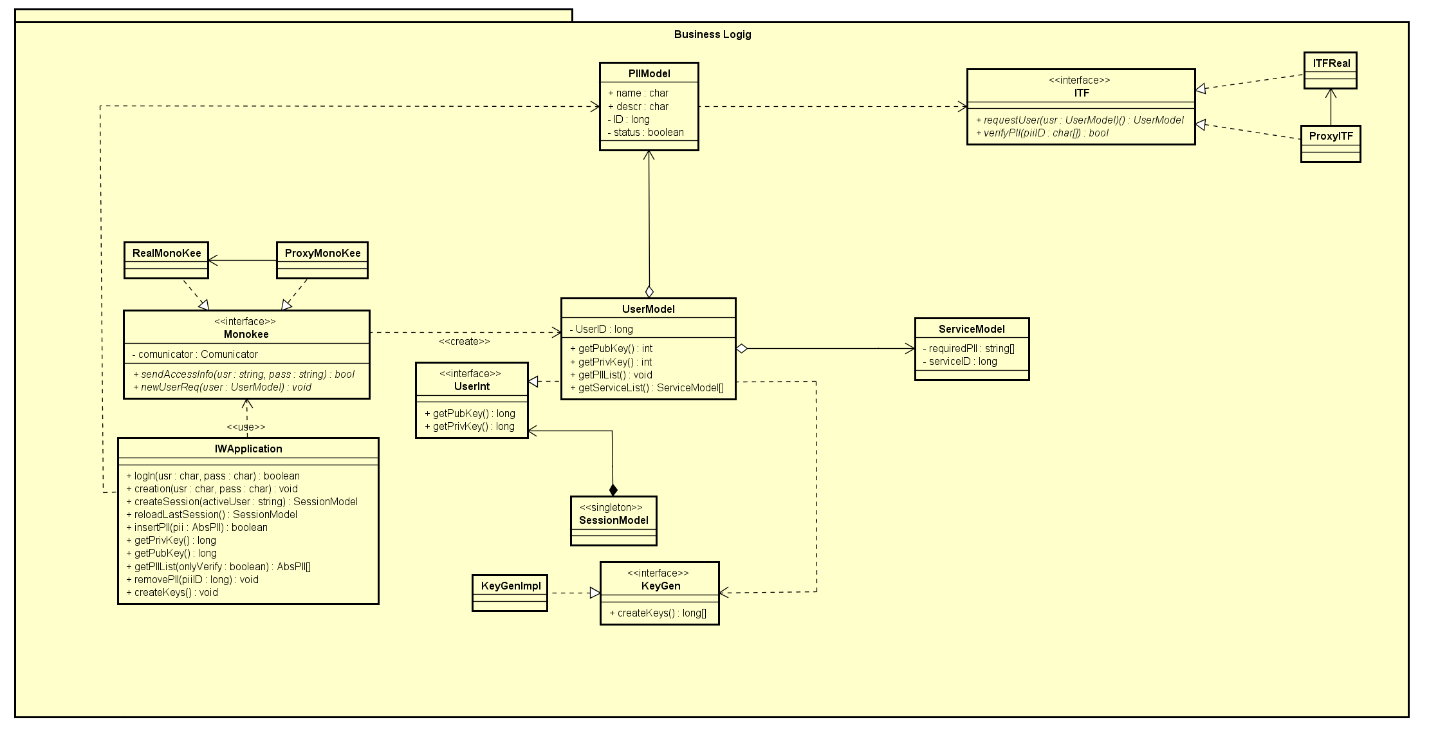
\includegraphics[width=0.9\columnwidth]{bl-lay-iw.png} 
    \caption{Diagramma BusinessLogic Layer IW}
    \label{fig:bl-lay-iw} 
\end{figure}

\paragraph{Monokee (interfaccia)}
Questa interfaccia rappresenta l’entità Monokee, con le classi RealMonokee e MonokeeProxy partecipa ad un’applicazione di un proxy pattern.

\paragraph{Metodi:}
\paragraph{Public async bool sendAccessInfo(userID: string, pass:string)}
        \begin{center}
            \begin{longtable}{|p{3cm}|p{9cm}|}%
            \caption{Public async bool sendAccessInfo(userID: string, pass:string)}
            \endfirsthead
            \endhead
            \hline
            \textbf{Descrizione} & Il metodo ha il compito di restituire true in caso i parametri passati corrispondano ad un username e una password di un utente presente nel servizio Monokee. False altrimenti. La chiamata è asincrona.\\
            \hline
            \textbf{Parametri} &      
            \begin{itemize}
                \item userID: stringa che rappresenta la chiave dell’utente
                \item pass: stringa che rappresenta la password dell’utente in chiaro.
            \end{itemize}
            \\
            \hline
            \textbf{Pseudo Codice} & 
            Non presente
            \\
            \hline
            \textbf{Note} & 
            -
            \\
            \hline
            \end{longtable}
            \end{center}




\paragraph{Public void newUserRequest(user:UserModel)}
\begin{center}
    \begin{longtable}{|p{3cm}|p{9cm}|}%
    \caption{Public void newUserRequest(user:UserModel)}
    \endfirsthead
    \endhead
    \hline
    \textbf{Descrizione} & Il metodo ha il compito di creare una richiesta di creazione utente in Monokee. Il metodo invia solo la richiesta, non ha modo di sapere se l’utente venga creato o meno.\\
    \hline
    \textbf{Parametri} &      
    \begin{itemize}
        \item user: è un riferimento ad un oggetto userModel che contiene i dati con cui si vuole inviare la richiesta di creazione l’utente.
    \end{itemize}
    \\
    \hline
    \textbf{Pseudo Codice} & 
    Non presente
    \\
    \hline
    \textbf{Note} & 
    -
    \\
    \hline
    \end{longtable}
    \end{center}



\paragraph{RealMonokee (implementa Monokee)}
Rappresenta una reale istanza del servizio Monokee. Con Monokee e MonokeeProxy rappresenta un’applicazione del pattern Proxy.
\paragraph{Campi dati:}
\begin{itemize}
    \item comunicator: è un riferimento di un oggetto che implementa l’interfaccia Comunicator.
\end{itemize}
\paragraph{Metodi:}




\paragraph{Public async bool sendAccessInfo (userID: string, pass:string)}
\begin{center}
    \begin{longtable}{|p{3cm}|p{9cm}|}%
    \caption{Public async bool sendAccessInfo (userID: string, pass:string)}
    \endfirsthead
    \endhead
    \hline
    \textbf{Descrizione} & Il metodo ha il compito di restituire true in caso i parametri passati corrispondano ad un username e una password di un utente presente nel servizio Monokee. False altrimenti.\\
    \hline
    \textbf{Parametri} &      
    \begin{itemize}
        \item userID: long che rappresenta la chiave dell’utente
        \item serviceID: long che rappresenta la chiave del servizio richiesto
    \end{itemize}
    \\
    \hline
    \textbf{Pseudo Codice} & 
    Return Async Communicator.verifyUserMonokee(userID,serviceID);
    \\
    \hline
    \textbf{Note} & 
    -
    \\
    \hline
    \end{longtable}
    \end{center}



\paragraph{Public void newUserRequest(user:UserModel)}
\begin{center}
    \begin{longtable}{|p{3cm}|p{9cm}|}%
    \caption{Public void newUserRequest(user:UserModel)}
    \endfirsthead
    \endhead
    \hline
    \textbf{Descrizione} & Il metodo ha il compito di creare una richiesta di creazione utente in Monokee. Il metodo invia solo la richiesta, non ha modo di sapere se l’utente venga creato o meno.\\
    \hline
    \textbf{Parametri} &      
    \begin{itemize}
        \item user: è un riferimento ad un oggetto userModel che contiene i dati con cui si vuole inviare la richiesta di creazione l’utente.
    \end{itemize}
    \\
    \hline
    \textbf{Pseudo Codice} & 
    Communicator.userCreationReq(user:UserModel);
    \\
    \hline
    \textbf{Note} & 
    -
    \\
    \hline
    \end{longtable}
    \end{center}


\paragraph{MonokeeProxy (implementa Monokee)}
Rappresenta un proxy remoto del servizio Monokee. Applica una politica di acquisizione pigra. Con Monokee e RealMonokee rappresenta un’applicazione del pattern Proxy.
\paragraph{Campi dati:}
\begin{itemize}
    \item realMonokee: è un riferimento di un oggetto RealMonokee.
\end{itemize}

\paragraph{Metodi:}

\paragraph{Public async bool sendAccessInfo (userID: string, pass:string)}
\begin{center}
    \begin{longtable}{|p{3cm}|p{9cm}|}%
    \caption{Public async bool sendAccessInfo (userID: string, pass:string)}
    \endfirsthead
    \endhead
    \hline
    \textbf{Descrizione} & Il metodo ha il compito di restituire true in caso i parametri passati corrispondano ad un username e una password di un utente presente nel servizio Monokee. False altrimenti.\\
    \hline
    \textbf{Parametri} &      
    \begin{itemize}
        \item userID: long che rappresenta la chiave dell’utente
        \item serviceID: long che rappresenta la chiave del servizio richiesto
    \end{itemize}
    \\
    \hline
    \textbf{Pseudo Codice} & 
    applyPolicy1;\newline
    applyPolicy2;\newline
    … \newline
    applyPolicyN;\newline
    realMonokee.sendAccessInfo(userID, pass);\newline
    \\
    \hline
    \textbf{Note} & 
    -
    \\
    \hline
    \end{longtable}
    \end{center}



\paragraph{Public void newUserRequest(user:UserModel)}
\begin{center}
    \begin{longtable}{|p{3cm}|p{9cm}|}%
    \caption{Public void newUserRequest(user:UserModel)}
    \endfirsthead
    \endhead
    \hline
    \textbf{Descrizione} & Il metodo ha il compito di creare una richiesta di creazione utente in Monokee. Il metodo invia solo la richiesta, non ha modo di sapere se l’utente venga creato o meno.\\
    \hline
    \textbf{Parametri} &      
    \begin{itemize}
        \item user: è un riferimento ad un oggetto userModel che contiene i dati con cui si vuole inviare la richiesta di creazione l’utente.
    \end{itemize}
    \\
    \hline
    \textbf{Pseudo Codice} & 
    applyPolicy1;\newline
    applyPolicy2;\newline
    …\newline
    applyPolicyN;\newline
    realMonokee.newUserRequest(user);\newline
    \\
    \hline
    \textbf{Note} & 
    -
    \\
    \hline
    \end{longtable}
    \end{center}



\paragraph{UserInt (interfaccia)}
Questa interfaccia definisce le caratteristiche minime che deve avere un utente generico dell’applicazione. Queste proprietà sono le chiavi private e pubbliche. UserModel implementa questa interfaccia. Questo ADT è stato pensato in un’ottica futura in cui ci potrebbero essere utenti non di Monokee.

\paragraph{Metodi:}
\paragraph{public void getPrivKey()}
\begin{center}
    \begin{longtable}{|p{3cm}|p{9cm}|}%
    \caption{public void getPrivKey()}
    \endfirsthead
    \endhead
    \hline
    \textbf{Descrizione} & Il metodo ha il compito ritornare la chiave privata presenta nella base di dati se presente. Se non presente genera la coppia e la ritorna.\\
    \hline
    \textbf{Parametri} &      
    -
    \\
    \hline
    \textbf{Pseudo Codice} & 
    Non presente
    \\
    \hline
    \textbf{Note} & 
    -
    \\
    \hline
    \end{longtable}
    \end{center}



\paragraph{public void getPubKey()}
\begin{center}
    \begin{longtable}{|p{3cm}|p{9cm}|}%
    \caption{public void getPubKey()}
    \endfirsthead
    \endhead
    \hline
    \textbf{Descrizione} & Il metodo ha il compito ritornare la chiave privata presenta nella base di dati se presente. Se non presente genera la coppia e la ritorna.\\
    \hline
    \textbf{Parametri} &      
    -
    \\
    \hline
    \textbf{Pseudo Codice} & 
    Non presente
    \\
    \hline
    \textbf{Note} & 
    -
    \\
    \hline
    \end{longtable}
    \end{center}

\paragraph{ServiceModel (implementa INotifyPropertyChanged)}
Questa classe rappresenta un servizio a cui l’utente può avere accesso. È definito dalla un codice e da una lista di PII richieste per effettuare l’accesso. Questo oggetto dovrà essere sempre generato da Monokee e mai salvato in locale. Questo al fine di evitare dati discordanti.
\paragraph{Campi dati:}
\begin{itemize}
    \item serviceID: è una stringa che rappresenta una chiave del servizio all’interno di Monokee.
    \item requiredPII[]: è un array di stringhe che rappresentano gli ID delle PII necessarie per effettuare il login al servizio identificato da serviceID
\end{itemize}

\paragraph{Metodi:}
Ogni attributo deve avere un \emph{getter} e un \emph{setter}, questi andranno implementati seguendo le funzionalità che offre C\#. Ogni \emph{setter} deve chiamare PropertyChanged al fine di garantire un corretto data binding.

\paragraph{private void PropertyChanged (propertyName)}
\begin{center}
    \begin{longtable}{|p{3cm}|p{9cm}|}%
    \caption{private void PropertyChanged (propertyName)}
    \endfirsthead
    \endhead
    \hline
    \textbf{Descrizione} & Il metodo ha il compito di effettuare il databinding con gli oggetti che modellano la vista e il database.\\
    \hline
    \textbf{Parametri} &      
    \begin{itemize}
        \item propertyName: il nome della variabile a cui è stato effettuato il cambiamento.
    \end{itemize}
    \\
    \hline
    \textbf{Pseudo Codice} & 
    this.PropertyChanged?.Invoke(this, 
    new PropertyChangedEventArgs(propertyName));
    \\
    \hline
    \textbf{Note} & 
    Questo metodo deve essere chiamato da ogni set presente nel seguente modo OnPropertyChanged(nameof(nome));
    \\
    \hline
    \end{longtable}
    \end{center}

\paragraph{Keygen (interfaccia)}
Questa interfaccia rappresenta un Strategy pattern per nascondere l’implementazione della reale libreria che effettua la generazione delle chiavi. Ha anche il compito di criptare e decriptare i dati.
\paragraph{Metodi:}
\paragraph{public long [] createKeys()}
\begin{center}
    \begin{longtable}{|p{3cm}|p{9cm}|}%
    \caption{public long [] createKeys()}
    \endfirsthead
    \endhead
    \hline
    \textbf{Descrizione} & Il metodo ha il compito di creare una coppia di chiavi pubbliche e private e quindi di restituirle. Ritorna un array di string di due elementi. Il primo elemento è la chiave pubblica, il secondo la privata.\\
    \hline
    \textbf{Parametri} &      
    -
    \\
    \hline
    \textbf{Pseudo Codice} & 
    Non presente.
    \\
    \hline
    \textbf{Note} & 
    -
    \\
    \hline
    \end{longtable}
    \end{center}



\paragraph{public long [] createKeys()}
\begin{center}
    \begin{longtable}{|p{3cm}|p{9cm}|}%
    \caption{public long [] createKeys()}
    \endfirsthead
    \endhead
    \hline
    \textbf{Descrizione} & Il metodo ha il compito di creare una coppia di chiavi pubbliche e private e quindi di restituirle. Ritorna un array di string di due elementi. Il primo elemento è la chiave pubblica, il secondo la privata.\\
    \hline
    \textbf{Parametri} &      
    -
    \\
    \hline
    \textbf{Pseudo Codice} & 
    Non presente.
    \\
    \hline
    \textbf{Note} & 
    -
    \\
    \hline
    \end{longtable}
    \end{center}



\paragraph{public static byte[] Encrypt(string publicKey, string data)}
\begin{center}
    \begin{longtable}{|p{3cm}|p{9cm}|}%
    \caption{public static byte[] Encrypt(string publicKey, string data)}
    \endfirsthead
    \endhead
    \hline
    \textbf{Descrizione} & Il metodo ha il compito di firmare i dati forniti con la chiave pubblica fornita.\\
    \hline
    \textbf{Parametri} &      
    \begin{itemize}
        \item publicKey: stringa che rappresenta la chiave pubblica
        \item Data: stringa che rappresenta i dati che si vogliono firmare
    \end{itemize}
    \\
    \hline
    \textbf{Pseudo Codice} & 
    Non presente.
    \\
    \hline
    \textbf{Note} & 
    -
    \\
    \hline
    \end{longtable}
    \end{center}



\paragraph{public static string Decrypt(string privateKey, byte[] encryptedBytes)}
\begin{center}
    \begin{longtable}{|p{3cm}|p{9cm}|}%
    \caption{public static string Decrypt(string privateKey, byte[] encryptedBytes)}
    \endfirsthead
    \endhead
    \hline
    \textbf{Descrizione} & Il metodo ha il compito di decriptare i dati forniti con la chiave privata fornita.\\
    \hline
    \textbf{Parametri} &      
    \begin{itemize}
        \item privateKey: stringa che rappresenta la chiave privata
        \item encryptedBytes: array di byte che rappresentano i dati che si vogliono decriptare.
    \end{itemize}
    \\
    \hline
    \textbf{Pseudo Codice} & 
    Non presente.
    \\
    \hline
    \textbf{Note} & 
    -
    \\
    \hline
    \end{longtable}
    \end{center}


\paragraph{KeygenImpl (implementa KeyGen)}
Questa interfaccia rappresenta un template pattern per nascondere l’implementazione della reale libreria che effettua la generazione delle chiavi.
\paragraph{Metodi:}

\paragraph{public static string Decrypt(string privateKey, byte[] encryptedBytes)}
\begin{center}
    \begin{longtable}{|p{3cm}|p{9cm}|}%
    \caption{public static string Decrypt(string privateKey, byte[] encryptedBytes)}
    \endfirsthead
    \endhead
    \hline
    \textbf{Descrizione} & Il metodo ha il compito di creare una coppia di chiavi pubbliche e private e quindi di restituirle. Ritorna un array di string di due elementi. Il primo elemento è la chiave pubblica, il secondo la privata.\\
    \hline
    \textbf{Parametri} &      
    -
    \\
    \hline
    \textbf{Pseudo Codice} & 
    CspParameters cspParams = new CspParameters { ProviderType = 1 };\newline

    RSACryptoServiceProvider rsaProvider = new RSACryptoServiceProvider(1024, cspParams);\newline

    string publicKey = Convert.ToBase64String(rsaProvider.ExportCspBlob(false));\newline
    string privateKey = Convert.ToBase64String(rsaProvider.ExportCspBlob(true));\newline

    return new array = {privateKey, publicKey};\newline
    \\
    \hline
    \textbf{Note} & 
    \url{https://stackoverflow.com/questions/18850030/aes-256-encryption-public-and-private-key-how-can-i-generate-and-use-it-net}
    \\
    \hline
    \end{longtable}
    \end{center}


\paragraph{public static byte[] Encrypt(string publicKey, string data)}
\begin{center}
    \begin{longtable}{|p{3cm}|p{9cm}|}%
    \caption{public static byte[] Encrypt(string publicKey, string data)}
    \endfirsthead
    \endhead
    \hline
    \textbf{Descrizione} & Il metodo ha il compito di firmare i dati forniti con la chiave pubblica fornita.\\
    \hline
    \textbf{Parametri} &      
    \begin{itemize}
        \item publicKey: stringa che rappresenta la chiave pubblica
        \item Data: stringa che rappresenta i dati che si vogliono firmare
    \end{itemize}
    \\
    \hline
    \textbf{Pseudo Codice} & 
    CspParameters cspParams = new CspParameters { ProviderType = 1 };\newline
    RSACryptoServiceProvider rsaProvider = new RSACryptoServiceProvider(cspParams);\newline
    rsaProvider.ImportCspBlob(Convert.FromBase64String(publicKey));\newline
    byte[] plainBytes = Encoding.UTF8.GetBytes(data);\newline
    byte[] encryptedBytes = rsaProvider.Encrypt(plainBytes, false);\newline
    return encryptedBytes;\newline
    \\
    \hline
    \textbf{Note} & 
    \url{https://stackoverflow.com/questions/18850030/aes-256-encryption-public-and-private-key-how-can-i-generate-and-use-it-net}
    \\
    \hline
    \end{longtable}
    \end{center}



\paragraph{public static string Decrypt(string privateKey, byte[] encryptedBytes)}
\begin{center}
    \begin{longtable}{|p{3cm}|p{9cm}|}%
    \caption{public static string Decrypt(string privateKey, byte[] encryptedBytes)}
    \endfirsthead
    \endhead
    \hline
    \textbf{Descrizione} & Il metodo ha il compito di decriptare i dati forniti con la chiave privata fornita.\\
    \hline
    \textbf{Parametri} &      
    \begin{itemize}
        \item privateKey: stringa che rappresenta la chiave privata
        \item encryptedBytes: array di byte che rappresentano i dati che si vogliono decriptare.
    \end{itemize}
    \\
    \hline
    \textbf{Pseudo Codice} & 
    CspParameters cspParams = new CspParameters { ProviderType = 1 };\item
    RSACryptoServiceProvider rsaProvider = new RSACryptoServiceProvider(cspParams);\item

    rsaProvider.ImportCspBlob(Convert.FromBase64String(privateKey));\item

    byte[] plainBytes = rsaProvider.Decrypt(encryptedBytes, false);\item

    string plainText = Encoding.UTF8.GetString(plainBytes, 0, plainBytes.Length);\item

    return plainText;\item
    \\
    \hline
    \textbf{Note} & 
    \url{https://stackoverflow.com/questions/18850030/aes-256-encryption-public-and-private-key-how-can-i-generate-and-use-it-net}
    \\
    \hline
    \end{longtable}
    \end{center}

\paragraph{ITF (interfaccia)}
Questa interfaccia rappresenta il componente ITF. Con RealITF e ITFProxy partecipano ad un’applicazione del Proxy Pattern.
\paragraph{Metodi:}


\paragraph{public verifyPII(pii: PIIModel[]):bool}
\begin{center}
    \begin{longtable}{|p{3cm}|p{9cm}|}%
    \caption{public verifyPII(pii: PIIModel[]):bool}
    \endfirsthead
    \endhead
    \hline
    \textbf{Descrizione} & Il metodo ha il compito di verificare presso l’ITF le informazioni PII. Il metodo si occupa della creazione dell’Hash.\\
    \hline
    \textbf{Parametri} &      
    \begin{itemize}
        \item pii: è una lista di oggetti PIIModel da verificare nell’ITF.
    \end{itemize}
    \\
    \hline
    \textbf{Pseudo Codice} & 
    Non presente.
    \\
    \hline
    \textbf{Note} & 
    -
    \\
    \hline
    \end{longtable}
    \end{center}



\paragraph{public requestUser(usr: userModel[]):bool}
\begin{center}
    \begin{longtable}{|p{3cm}|p{9cm}|}%
    \caption{public requestUser(usr: userModel[]):bool}
    \endfirsthead
    \endhead
    \hline
    \textbf{Descrizione} & Il metodo ha il compito creare un utente all’interno dell’ITF.\\
    \hline
    \textbf{Parametri} &      
    \begin{itemize}
        \item usr: rappresenta l’utente che si vuole immettere nell’ITF
    \end{itemize}
    \\
    \hline
    \textbf{Pseudo Codice} & 
    Non presente.
    \\
    \hline
    \textbf{Note} & 
    La chiave pubblica rappresenta l’ID dell’utente.
    \\
    \hline
    \end{longtable}
    \end{center}

\paragraph{RealITF (implementa ITF)}
Questa interfaccia rappresenta il reale componente ITF. Si occupa di instaurare la comunicazione tramite l’uso di un BlockchainClient. Con ITF e ITFProxy partecipano ad un’applicazione del Proxy Pattern.

\paragraph{Campi dati:}
tutti gli oggetti necessari vengono ottenuti tramite l’uso del DependencyService.

\paragraph{Metodi:}

\paragraph{public verifyPII(pii: PIIModel []):bool}
\begin{center}
    \begin{longtable}{|p{3cm}|p{9cm}|}%
    \caption{public verifyPII(pii: PIIModel []):bool}
    \endfirsthead
    \endhead
    \hline
    \textbf{Descrizione} & Il metodo ha il compito di verificare presso l’ITF le informazioni PII\\
    \hline
    \textbf{Parametri} &      
    \begin{itemize}
        \item pii: è una lista di oggetti hashedPII da verificare nell’ITF.
    \end{itemize}
    \\
    \hline
    \textbf{Pseudo Codice} & 
    Var blockClient = DependencyService.Get<BlockchainClient>();\newline
    HashAlgorithm algorithm = SHA256.Create();\newline
    Var hasedDesc = algorithm.ComputeHash(Encoding.UTF8.GetBytes(pii.desc));\newline
    Var hashedName = algorithm.ComputeHash(Encoding.UTF8.GetBytes(pii.name));\newline

    Return blockClient.createID(piiModel.id,hashedName, hashedDesc);\newline
    \\
    \hline
    \textbf{Note} & 
    -
    \\
    \hline
    \end{longtable}
    \end{center}



\paragraph{public bool requestUser(usr: userModel[])}
\begin{center}
    \begin{longtable}{|p{3cm}|p{9cm}|}%
    \caption{public bool requestUser(usr: userModel[])}
    \endfirsthead
    \endhead
    \hline
    \textbf{Descrizione} & Il metodo ha il compito creare un utente all’interno dell’ITF.\\
    \hline
    \textbf{Parametri} &      
    \begin{itemize}
        \item usr: rappresenta l’utente che si vuole immettere nell’ITF
    \end{itemize}
    \\
    \hline
    \textbf{Pseudo Codice} & 
    Var blockClient = DependencyService.Get<BlockchainClient>();\newline
    Return blockClient.createID(usr.getPublicKey());\newline
    \\
    \hline
    \textbf{Note} & 
    La chiave pubblica rappresenta l’ID dell’utente.
    \\
    \hline
    \end{longtable}
    \end{center}

\paragraph{ITFProxy (implementa ITF)}
Questa interfaccia rappresenta un remote proxy del componente ITF. Si occupa applicare una serie di politiche. Con ITF e ITFProxy partecipano ad un’applicazione del Proxy Pattern.
\paragraph{Campi dati:}
\begin{itemize}
    \item realITF: è un riferimento ad un oggetto RealITF. 
\end{itemize}



\paragraph{Metodi:}

\paragraph{public verifyPII(pii: PIIModel []):bool}
\begin{center}
    \begin{longtable}{|p{3cm}|p{9cm}|}%
    \caption{public verifyPII(pii: PIIModel []):bool}
    \endfirsthead
    \endhead
    \hline
    \textbf{Descrizione} & Il metodo ha il compito di verificare presso l’ITF le informazioni PII\\
    \hline
    \textbf{Parametri} &      
    \begin{itemize}
        \item pii: è una lista di oggetti hashedPII da verificare nell’ITF.
    \end{itemize}
    \\
    \hline
    \textbf{Pseudo Codice} & 
    Return realITF.verifyPII(pii);
    \\
    \hline
    \textbf{Note} & 
    -
    \\
    \hline
    \end{longtable}
    \end{center}



\paragraph{public bool requestUser(usr: userModel[])}
\begin{center}
    \begin{longtable}{|p{3cm}|p{9cm}|}%
    \caption{public bool requestUser(usr: userModel[])}
    \endfirsthead
    \endhead
    \hline
    \textbf{Descrizione} & Il metodo ha il compito creare un utente all’interno dell’ITF.\\
    \hline
    \textbf{Parametri} &      
    \begin{itemize}
        \item usr: rappresenta l’utente che si vuole immettere nell’ITF
    \end{itemize}
    \\
    \hline
    \textbf{Pseudo Codice} & 
    realITF. requestUser(usr: userModel[]);
    \\
    \hline
    \textbf{Note} & 
    La chiave pubblica rappresenta l’ID dell’utente.
    \\
    \hline
    \end{longtable}
    \end{center}

\paragraph{IWApplication}
Questa classe rappresenta un facade che espone tutte le funzioni che può compiere un utente attraverso le varie viste.
\paragraph{Campi dati:}
\begin{itemize}
    \item monokee: è un riferimento ad un oggetto che implementa l’interfaccia Monokee.
    \item database: è un riferimento ad un oggetto DBDao ottenuto tramite l’uso di DependecyService.
\end{itemize}

\paragraph{Metodi:}

\paragraph{public bool logIn(usr: string, pass:string)}
\begin{center}
    \begin{longtable}{|p{3cm}|p{9cm}|}%
    \caption{public bool logIn(usr: string, pass:string)}
    \endfirsthead
    \endhead
    \hline
    \textbf{Descrizione} & Il metodo ha il compito di verificare che le credenziali fornite dall’utente corrispondano anche nel servizio Monokee.\\
    \hline
    \textbf{Parametri} &      
    \begin{itemize}
        \item  usr: rappresenta la chiave dell’utente
        \item Pass: è una stringa che rappresenta la password dell’utente
    \end{itemize}
    \\
    \hline
    \textbf{Pseudo Codice} & 
    Var b = Monokee.sendAccessInfo(usr, pass);\newline
    Return b;\newline
    \\
    \hline
    \textbf{Note} & 
    -
    \\
    \hline
    \end{longtable}
    \end{center}


\paragraph{public void creation(usr: string, pass:string)}
\begin{center}
    \begin{longtable}{|p{3cm}|p{9cm}|}%
    \caption{public void creation(usr: string, pass:string)}
    \endfirsthead
    \endhead
    \hline
    \textbf{Descrizione} & Il metodo ha il compito di inviare una richiesta di creazione utente di un utente. Questo metodo invia solo una richiesta, non a modo di sapere se l’utente verrà effettivamente creato.\\
    \hline
    \textbf{Parametri} &      
    \begin{itemize}
        \item  usr: rappresenta la chiave dell’utente
        \item Pass: è una stringa che rappresenta la password dell’utente
    \end{itemize}
    \\
    \hline
    \textbf{Pseudo Codice} & 
    Var b = Monokee.newUserRequest(usr, pass);\newline
    Return b;\newline
    \\
    \hline
    \textbf{Note} & 
    -
    \\
    \hline
    \end{longtable}
    \end{center}


\paragraph{public void createSession(activeUser: string)}
\begin{center}
    \begin{longtable}{|p{3cm}|p{9cm}|}%
    \caption{public void createSession(activeUser: string)}
    \endfirsthead
    \endhead
    \hline
    \textbf{Descrizione} & Il metodo ha il compito creare la sessione e di inserirla nel database come lastSession.\\
    \hline
    \textbf{Parametri} &      
    \begin{itemize}
        \item  usr: rappresenta la chiave dell’utente
        \item Pass: è una stringa che rappresenta la password dell’utente
    \end{itemize}
    \\
    \hline
    \textbf{Pseudo Codice} & 
    currentSession = new SessionModel(activeUser.id);\newline
    App.currentSession = currentSession;\newline
    Database.saveCurrentSession();\newline
    \\
    \hline
    \textbf{Note} & 
    La current session è mantenuta nell’oggetto App.
    \\
    \hline
    \end{longtable}
    \end{center}



\paragraph{public void reloadLastSession()}
\begin{center}
    \begin{longtable}{|p{3cm}|p{9cm}|}%
    \caption{public void reloadLastSession()}
    \endfirsthead
    \endhead
    \hline
    \textbf{Descrizione} & Il metodo ha il compito ricaricare l’ultima sessione dal database e ritornala.\\
    \hline
    \textbf{Parametri} &      
    \begin{itemize}
        \item  usr: rappresenta la chiave dell’utente
        \item Pass: è una stringa che rappresenta la password dell’utente
    \end{itemize}
    \\
    \hline
    \textbf{Pseudo Codice} & 
    Return database.getLastSession();
    \\
    \hline
    \textbf{Note} & 
    -
    \\
    \hline
    \end{longtable}
    \end{center}



\paragraph{public void insertPII(pii:PIIModel)}
\begin{center}
    \begin{longtable}{|p{3cm}|p{9cm}|}%
    \caption{public void insertPII(pii:PIIModel)}
    \endfirsthead
    \endhead
    \hline
    \textbf{Descrizione} & Il metodo ha il compito inserire la pii all’utente corrente e anche all’interno dell’ITF.\\
    \hline
    \textbf{Parametri} &      
    \begin{itemize}
        \item pii: rappresenta la PII che si vuole inserire all’utente corrente
    \end{itemize}
    \\
    \hline
    \textbf{Pseudo Codice} & 
    Database.addPII(pii,status = false)\newline
    BlockchainClient.addPII\newline
    (App.currentSession.activeUser, pii);\newline
    \\
    \hline
    \textbf{Note} & 
    \\
    \hline
    \end{longtable}
    \end{center}

    \paragraph{public void getPrivKey()}
    \begin{center}
        \begin{longtable}{|p{3cm}|p{9cm}|}%
        \caption{public void getPrivKey()}
        \endfirsthead
        \endhead
        \hline
        \textbf{Descrizione} & Il metodo ha il compito ritornare la chiave privata dell’utente che indicato come active user nella sessione corrente.\\
        \hline
        \textbf{Parametri} &      
        \begin{itemize}
            \item pii: rappresenta la PII che si vuole inserire all’utente corrente
        \end{itemize}
        \\
        \hline
        \textbf{Pseudo Codice} & 
        Return BlockchainClient\newline
        .addPII(App.currentSession\newline
        .activeUser.getPrivKey();\newline
        \\
        \hline
        \textbf{Note} & 
        -
        \\
        \hline
        \end{longtable}
        \end{center}
    
\paragraph{public void getPubKey()}
\begin{center}
    \begin{longtable}{|p{3cm}|p{9cm}|}%
    \caption{public void getPubKey()}
    \endfirsthead
    \endhead
    \hline
    \textbf{Descrizione} & Il metodo ha il compito ritornare la chiave Pubblica dell’utente che indicato come active user nella sessione corrente.\\
    \hline
    \textbf{Parametri} &      
    \begin{itemize}
        \item pii: rappresenta la PII che si vuole inserire all’utente corrente
    \end{itemize}
    \\
    \hline
    \textbf{Pseudo Codice} & 
    Return BlockchainClient\newline
    .addPII(App.currentSession\newline
    .activeUser.getPUBKey();\newline
    \\
    \hline
    \textbf{Note} & 
    -
    \\
    \hline
    \end{longtable}
\end{center}

\paragraph{public void getPIIList()}
\begin{center}
    \begin{longtable}{|p{3cm}|p{9cm}|}%
    \caption{public void getPIIList()}
    \endfirsthead
    \endhead
    \hline
    \textbf{Descrizione} & Il metodo ha il compito ritornare la lista di PII dell’utente che è indicato come active user nella sessione corrente.\\
    \hline
    \textbf{Parametri} &      
    \begin{itemize}
        \item pii: rappresenta la PII che si vuole inserire all’utente corrente
    \end{itemize}
    \\
    \hline
    \textbf{Pseudo Codice} & 
    Return \newline
    App.currentSession \newline
    .activeUser.getPIIList(); \newline
    \\
    \hline
    \textbf{Note} & 
    -
    \\
    \hline
    \end{longtable}
\end{center}

\paragraph{public void removePII(pii:string)}
\begin{center}
    \begin{longtable}{|p{3cm}|p{9cm}|}%
    \caption{public void removePII(pii:string)}
    \endfirsthead
    \endhead
    \hline
    \textbf{Descrizione} & Il metodo ha il compito inserire la pii all’utente corrente e anche all’interno dell’ITF.\\
    \hline
    \textbf{Parametri} &      
    \begin{itemize}
        \item pii: rappresenta la chiave dellla PII che si vuole inserire all’utente corrente
    \end{itemize}
    \\
    \hline
    \textbf{Pseudo Codice} & 
    Database.removePII(pii,status = false)\newline
    BlockchainClient.removePII(pii);\newline
    \\
    \hline
    \textbf{Note} & 
    -
    \\
    \hline
    \end{longtable}
\end{center}



\paragraph{public Tuple<string,string> createKeys()}
\begin{center}
    \begin{longtable}{|p{3cm}|p{9cm}|}%
    \caption{public Tuple<string,string> createKeys()}
    \endfirsthead
    \endhead
    \hline
    \textbf{Descrizione} & Il metodo ha il compito di creare all’utente corrente un paio di chiavi asincrone.\\
    \hline
    \textbf{Parametri} &      
    \begin{itemize}
        \item pii: rappresenta la chiave dellla PII che si vuole inserire all’utente corrente
    \end{itemize}
    \\
    \hline
    \textbf{Pseudo Codice} & 
    Var a = BlockchainClient \newline
    .addPII(App.currentSession.activeUser.getPriv(); \newline
    Var b = BlockchainClient \newline
    .addPII(App.currentSession.activeUser.getPubl(); \newline
    Return new Tuple<string,string>(a,b); \newline
    \\
    \hline
    \textbf{Note} & 
    L’algoritmo usato è SHA3 per questione di compatibilità con l'ITF.
    \\
    \hline
    \end{longtable}
\end{center}

\paragraph{IQRGenerator (interfaccia)}
Questa interfaccia rappresenta uno strategy Pattern per accomunare le varie implementazioni di algoritmi che generano una lista di byte che rappresentano immagini di codici QR.
\paragraph{Metodi:}

\paragraph{public byte[] generateQR(value: string)}
\begin{center}
    \begin{longtable}{|p{3cm}|p{9cm}|}%
    \caption{public byte[] generateQR(value: string)}
    \endfirsthead
    \endhead
    \hline
    \textbf{Descrizione} & Il metodo ha il compito di creare un’array di byte che rappresentano un’immagine del codice QR contenente la stringa definita in value.\\
    \hline
    \textbf{Parametri} &      
    \begin{itemize}
        \item value: è una stringa che rappresenta il testo che si vuole inserire dentro il QR.
    \end{itemize}
    \\
    \hline
    \textbf{Pseudo Codice} & 
    Non presente
    \\
    \hline
    \textbf{Note} & 
    -
    \\
    \hline
    \end{longtable}
\end{center}

\paragraph{IQRGenerator (implementa IQRgenerator)}
Questa classe rappresenta un’implementazione dell’algoritmo di generazione QR per Android.
\paragraph{Metodi:}

\paragraph{public byte[] generateQR(value: string)}
\begin{center}
    \begin{longtable}{|p{3cm}|p{9cm}|}%
    \caption{public byte[] generateQR(value: string)}
    \endfirsthead
    \endhead
    \hline
    \textbf{Descrizione} & Il metodo ha il compito di creare un’array di byte che rappresentano un’immagine del codice QR contenente la stringa definita in value.\\
    \hline
    \textbf{Parametri} &      
    \begin{itemize}
        \item value: è una stringa che rappresenta il testo che si vuole inserire dentro il QR.
    \end{itemize}
    \\
    \hline
    \textbf{Pseudo Codice} & 
    var writer = \newline
    new BarcodeWriter \newline
    \{\newline
        Format = BarcodeFormat.QRCODE,\newline
        Options = new EncodingOptions\newline
        \{\newline
            Height = 1600,\newline
            Width = 1600\newline
        \}\newline
    \};\newline
    Android.Graphics.Bitmap bm =  writer.Write(value);\newline
    MemoryStream stream = new MemoryStream();\newline
    bm.Compress(Bitmap.CompressFormat.Jpeg, 100, stream);\newline
    var arr =  stream.ToArray();\newline
    stream.Close();\newline
    return arr;\newline
    \\
    \hline
    \textbf{Note} & 
    -
    \\
    \hline
    \end{longtable}
\end{center}


\subsubsection{VM Layer}
Questo layer contiene i vari controllori che gestiscono le viste. Si è previsto di creare un controller per ogni pagina dell’applicazione. L’applicazione utilizza il pattern MVVM, quindi, i controlli sono delle ViewModel (VM) che contengono i dati e le operazioni. Tra i dati e la vista sono presenti dei binding da realizzare utilizzando gli strumenti forniti da Xamarin. Le VM operano le loro azioni tramite l’utilizzo della classe IWFacade. 

Esiste un controllore per ogni vista prevista dall’applicazione. Le seguenti sono:
\begin{itemize}
    \item LoginPageVM;
    \item MenuVM;
    \item ServiceListVM;
    \item ServicePageVM;
    \item PIIListVM;
    \item PIIPage;
    \item AddPIIPageVM.
\end{itemize}
Tutte queste classi devono estendere da INotifyPropertyChanged.
In figura \ref{fig:vm-layer-iw} il diagramma esplicativo del \emph{layer}.

\begin{figure}[htbp]
    \centering
    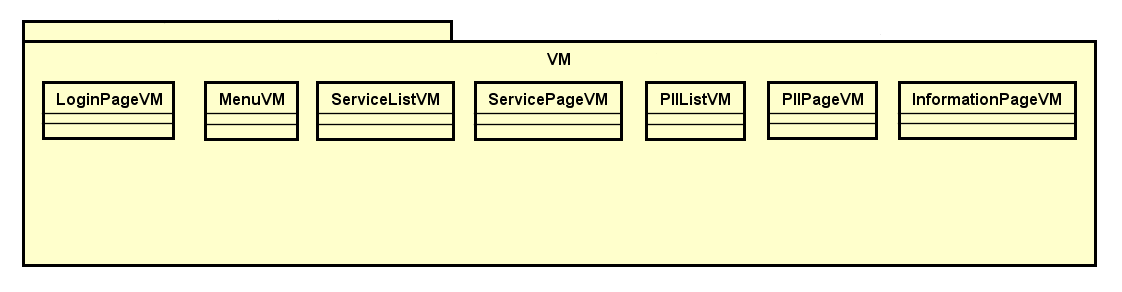
\includegraphics[width=0.9\columnwidth]{VMlayer-iw.png} 
    \caption{Diagramma UML VM Layer}
    \label{fig:vm-layer-iw} 
\end{figure}

\paragraph{LoginPageVM (implementa INotifyPropertyChanged)}
È il controllore della pagina di login.
\paragraph{Campi dati:}
\begin{itemize}
    \item DisplayInvalidLoginPrompt: è un rifermento ad un oggetto Action (Xamarin) che definisce l’azione da intaprendere in caso di credenziali errate. Questo oggetto è definito nel code-behind della vista e deve essere richiamato tramite una delegate.
    \item PropertyChanged: è un riferimento ad un oggetto Event (Xamarin).
    \item email: è una stringa in databing con la form presente nella vista. 
    \item password: è una stringa in databing con la form presente nella vista.
    \item SubmitCommand: e un riferimento ad un oggeto ICommand(Xamarin). Deve avere setter e getter pubblici.
\end{itemize}

I campi dati email, password devono avere i \emph{getter} e \emph{setter} tipici di C\#. Il \emph{setter} deve chiamare l’evento \emph{PropertyChanged}.

\paragraph{Metodi:}
\paragraph{public void OnSubmit()}
\begin{center}
    \begin{longtable}{|p{3cm}|p{9cm}|}%
    \caption{public void OnSubmit()}
    \endfirsthead
    \endhead
    \hline
    \textbf{Descrizione} & Il metodo ha il compito definire le procedure da intraprendere la verifica di email e password.\\
    \hline
    \textbf{Parametri} &      
    -
    \\
    \hline
    \textbf{Pseudo Codice} & 
    Var result = App.IWFacade.LogIn(email, password);\newline
    If result \{\newline
        Navigation.PushAsync (new ServiceListPage());\newline
    \}\newline
    Else DisplayInvalidLoginPrompt();\newline
    \\
    \hline
    \textbf{Note} & 
    \url{https://www.c-sharpcorner.com/article/xamarin-forms-create-a-login-page-mvvm/}
    \\
    \hline
    \end{longtable}
\end{center}


\paragraph{Metodi:}
\paragraph{public void OnSubmit()}
\begin{center}
    \begin{longtable}{|p{3cm}|p{9cm}|}%
    \caption{public void OnSubmit()}
    \endfirsthead
    \endhead
    \hline
    \textbf{Descrizione} & Il metodo ha il compito di eseguire le operazioni che portano al cambio della pagina in InfoPage.\\
    \hline
    \textbf{Parametri} &      
    -
    \\
    \hline
    \textbf{Pseudo Codice} & 
    Navigation.PushAsync (new InfoPage());
    \\
    \hline
    \textbf{Note} & 
    \url{https://www.c-sharpcorner.com/article/xamarin-forms-create-a-login-page-mvvm/}
    \\
    \hline
    \end{longtable}
\end{center}


\paragraph{MenuVM (implementa INotifyPropertyChanged)}
È il controllore del menu visualizzato nelle MasterDetaildePage
\paragraph{Campi dati:}
\begin{itemize}
    \item PropertyChanged: è un riferimento ad un oggetto Event (Xamarin).
    \item email: è una stringa in databing, da visualizzare per mostrare l’active user attuale. 
\end{itemize}
Il campo dati email deve avere i \emph{getter} e \emph{setter} tipici di C\#. Il \emph{setter} deve chiamare l’evento \emph{PropertyChanged}.

\paragraph{Metodi:}

\paragraph{Metodi:}
\paragraph{public void OnClickPIIList()}
\begin{center}
    \begin{longtable}{|p{3cm}|p{9cm}|}%
    \caption{public void OnClickPIIList()}
    \endfirsthead
    \endhead
    \hline
    \textbf{Descrizione} & Il metodo ha il compito di eseguire le operazioni che portano al cambio della pagina in PIIListPage.\\
    \hline
    \textbf{Parametri} &      
    -
    \\
    \hline
    \textbf{Pseudo Codice} & 
    Navigation.PushAsync (new PIIListPage());
    \\
    \hline
    \textbf{Note} & 
    -
    \\
    \hline
    \end{longtable}
\end{center}



\paragraph{public void OnClickKeys()}
\begin{center}
    \begin{longtable}{|p{3cm}|p{9cm}|}%
    \caption{public void OnClickKeys()}
    \endfirsthead
    \endhead
    \hline
    \textbf{Descrizione} & Il metodo ha il compito di eseguire le operazioni che portano al cambio della pagina in KeysPage.\\
    \hline
    \textbf{Parametri} &      
    -
    \\
    \hline
    \textbf{Pseudo Codice} & 
    Navigation.PushAsync (new KeysPage());
    \\
    \hline
    \textbf{Note} & 
    -
    \\
    \hline
    \end{longtable}
\end{center}



\paragraph{public void OnClickInfoPage()}
\begin{center}
    \begin{longtable}{|p{3cm}|p{9cm}|}%
    \caption{public void OnClickInfoPage()}
    \endfirsthead
    \endhead
    \hline
    \textbf{Descrizione} & Il metodo ha il compito di eseguire le operazioni che portano al cambio della pagina in InfoPage.\\
    \hline
    \textbf{Parametri} &      
    -
    \\
    \hline
    \textbf{Pseudo Codice} & 
    Navigation.PushAsync (new InfoPage());
    \\
    \hline
    \textbf{Note} & 
    -
    \\
    \hline
    \end{longtable}
\end{center}

\paragraph{KeysPageVM (implementa INotifyPropertyChanged)}
È il controllore della pagina che mostra le chiavi pubbliche e private.
\paragraph{Campi dati:}
\begin{itemize}
    \item PropertyChanged: è un riferimento ad un oggetto Event (Xamarin).
    \item email: è una stringa in databing, da visualizzare per mostrare l’active user attuale. 
    \item keyPriv: è una stringa in databing, da visualizzare per mostrare la chiave privata dell’active user attuale. 
    \item keyPub: è una stringa in databing, da visualizzare per mostrare la chiave pubblica dell’active user attuale. 
\end{itemize}

Il campo dati email, keyPriv, keyPub deve avere i \emph{getter} e \emph{setter} tipici di C\#. Il \emph{setter} deve chiamare l’evento \emph{PropertyChanged}.


\paragraph{Metodi:}
Questa pagina non prevede interazione con l’utente, quindi non prevede metodi.

\paragraph{PiiListVM (implementa INotifyPropertyChanged)}
È il controllore della pagina che mostra la lista dei servizi disponibili.
\paragraph{Campi dati:}
\begin{itemize}
    \item PropertyChanged: è un riferimento ad un oggetto Event (Xamarin).
    \item email: è una stringa in databing, da visualizzare per mostrare l’active user attuale. 
    \item piiList: è una lista di oggetti piiModel in databing con la vista.
\end{itemize}

Il campo dati email deve avere i \emph{getter} e \emph{setter} tipici di C\#. Il \emph{setter} deve chiamare l’evento \emph{PropertyChanged}.
\paragraph{Metodi:}



\paragraph{public void OnClickPII(piiID:string)}
\begin{center}
    \begin{longtable}{|p{3cm}|p{9cm}|}%
    \caption{public void OnClickPII(piiID:string)}
    \endfirsthead
    \endhead
    \hline
    \textbf{Descrizione} & Il metodo ha il compito di eseguire le operazioni che portano al cambio della pagina in PIIPage.\\
    \hline
    \textbf{Parametri} &      
    \begin{itemize}
        \item piiID: è una stringa che rappresenta la chiave della PII che ha generato l’evento.
    \end{itemize}
    \\
    \hline
    \textbf{Pseudo Codice} & 
    Navigation.PushAsync (new PIIPage(piiID));
    \\
    \hline
    \textbf{Note} & 
    -
    \\
    \hline
    \end{longtable}
\end{center}




\paragraph{ServiceListVM (implementa INotifyPropertyChanged)}
È il controllore della pagina che mostra la lista dei servizi disponibili.
\paragraph{Campi dati:}
\begin{itemize}
    \item PropertyChanged: è un riferimento ad un oggetto Event (Xamarin).
    \item email: è una stringa in databing, da visualizzare per mostrare l’active user attuale. 
    \item serviceList: è una lista di oggetti ServiceModel in databing con la vista.
\end{itemize}

Il campo dati email deve avere i \emph{getter} e \emph{setter} tipici di C\#. Il \emph{setter} deve chiamare l’evento \emph{PropertyChanged}.
\paragraph{Metodi:}




\paragraph{public void OnClickService(piiID:string)}
\begin{center}
    \begin{longtable}{|p{3cm}|p{9cm}|}%
    \caption{public void OnClickService(piiID:string)}
    \endfirsthead
    \endhead
    \hline
    \textbf{Descrizione} & Il metodo ha il compito di eseguire le operazioni che portano al cambio della pagina in ServicePage.\\
    \hline
    \textbf{Parametri} &      
    \begin{itemize}
        \item serviceID: è una stringa che rappresenta la chiave del  servizio che ha generato l’evento.
    \end{itemize}
    \\
    \hline
    \textbf{Pseudo Codice} & 
    Navigation.PushAsync (new ServicePage(serviceID));
    \\
    \hline
    \textbf{Note} & 
    -
    \\
    \hline
    \end{longtable}
\end{center}



\paragraph{PIIPageVM (implementa INotifyPropertyChanged)}
È il controllore della pagina che mostra la lista dei servizi disponibili.
\paragraph{Campi dati:}
\begin{itemize}
    \item PropertyChanged: è un riferimento ad un oggetto Event (Xamarin).
    \item piiID: è una stringa che rappresenta la chiave della pii da visualizzare, deve essere passata tramite il costruttore dell’oggetto e messa in databing con la vista.
    \item email: è una stringa in databing, da visualizzare per mostrare l’active user attuale. 
    \item Pii: è un riferimento ad un oggetto PIIModel che contiene I dati relative alla PII identificata dal piiID fornito nel costruttore. Le informazioni sono visualizzate nella vista.
\end{itemize}

Il campo dati email deve avere i \emph{getter} e \emph{setter} tipici di C\#. Il \emph{setter} deve chiamare l’evento \emph{PropertyChanged}.

\paragraph{Metodi:}
\paragraph{public void OnRemovePII(piiID:string)}
\begin{center}
    \begin{longtable}{|p{3cm}|p{9cm}|}%
    \caption{public void OnRemovePII(piiID:string)}
    \endfirsthead
    \endhead
    \hline
    \textbf{Descrizione} & Il metodo ha il compito rimuove la pii a cui fa riferimento la pagina.\\
    \hline
    \textbf{Parametri} &      
    \begin{itemize}
        \item PiiID: è una stringa che rappresenta la chiave della PII che si vuole eliminare.
    \end{itemize}
    \\
    \hline
    \textbf{Pseudo Codice} & 
    App.IWApplication.removePII(piiID);\newline
    Navigation.PushAsync (new PIIListPage(piiID));\newline
    \\
    \hline
    \textbf{Note} & 
    -
    \\
    \hline
    \end{longtable}
\end{center}




\paragraph{ServicePage (implementa INotifyPropertyChanged)}
È il controllore della pagina che mostra la lista dei servizi disponibili.
\paragraph{Campi dati:}
\begin{itemize}
    \item PropertyChanged: è un riferimento ad un oggetto Event (Xamarin).
    \item serviceID: è una stringa che rappresenta la chiave del Servizio da visualizzare, deve essere passata tramite il costruttore dell’oggetto e messa in databing con la vista.
    \item email: è una stringa in databing, da visualizzare per mostrare l’active user attuale. 
    \item serviceModel: è un riferimento ad un oggetto ServiceModel che contiene I dati relative alla PII identificata dal serviceID fornito nel costruttore. Le informazioni sono visualizzate nella vista.
\end{itemize}

Il campo dati email deve avere i \emph{getter} e \emph{setter} tipici di C\#. Il \emph{setter} deve chiamare l’evento \emph{PropertyChanged}.
\paragraph{Metodi:}

\paragraph{private void showQR(serviceID:string)}
\begin{center}
    \begin{longtable}{|p{3cm}|p{9cm}|}%
    \caption{private void showQR(serviceID:string)}
    \endfirsthead
    \endhead
    \hline
    \textbf{Descrizione} & Il metodo ha il compito mostrare nell’applicazione il QR con le informazioni necessarie per effettuare il login al servizio.\\
    \hline
    \textbf{Parametri} &      
    \begin{itemize}
        \item serviceID: è una stringa che rappresenta la chiave della PII che si vuole eliminare.
    \end{itemize}
    \\
    \hline
    \textbf{Pseudo Codice} & 
    Var services = App.currentSession.activeUser.getServiceList;\newline
    Var ser = Services[serviceID];\newline
    If ser != null \{\newline
    s = serviceName.toString() + ser.requiredPII;\newline
    \}\newline
    var qrwr = DependencyService.Get<Iqr>();\newline
    s = qrwr.GenQR(stringaInfo);\newline
    imaInVista.Source = ImageSource.FromStream(()=>new MemoryStream(s));\newline
    \\
    \hline
    \textbf{Note} & 
    -
    \\
    \hline
    \end{longtable}
\end{center}




\paragraph{AddPIIPageVM (implementa INotifyPropertyChanged)}
È il controllore della pagina di login.
\paragraph{Campi dati:}
\begin{itemize}
    \item PropertyChanged: è un riferimento ad un oggetto Event (Xamarin).
    \item piiName: è una stringa in databing con la form presente nella vista. 
    \item piiDesc: è una stringa in databing con la form presente nella vista.
    \item SubmitCommand: e un riferimento ad un oggeto ICommand(Xamarin). Deve avere setter e getter pubblici.
\end{itemize}

I campi dati email, password devono avere i \emph{getter} e \emph{setter} tipici di C\#. Il \emph{setter} deve chiamare l’evento \emph{PropertyChanged}.
\paragraph{Metodi:}

\paragraph{public void OnSubmit()}
\begin{center}
    \begin{longtable}{|p{3cm}|p{9cm}|}%
    \caption{public void OnSubmit()}
    \endfirsthead
    \endhead
    \hline
    \textbf{Descrizione} & Il metodo ha il compito definire le procedure da intraprendere per inserire la PII sia nella base di dati, sia nell’ITF\\
    \hline
    \textbf{Parametri} &      
    -
    \\
    \hline
    \textbf{Pseudo Codice} & 
    Var pii = new AbsPII(piiName, piiDesc);\newline
    Var result = App.IWApplication.insertPII(pii);\newline
    If result \{\newline
        Navigation.PushAsync (new PIIListPage());\newline
    \}\newline
    Else displayAllertError();\newline
    \\
    \hline
    \textbf{Note} & 
    -
    \\
    \hline
    \end{longtable}
\end{center}